\documentclass[11pt]{article}

\usepackage[a4paper,margin=1in]{geometry}
\usepackage{graphicx}
\usepackage{booktabs}
\usepackage{longtable}
\usepackage{pdflscape}
\usepackage{array}
\usepackage{tabularx}
\usepackage{hyperref}
\usepackage{natbib}
\usepackage{setspace}
\usepackage{float}
\usepackage{xcolor}
\usepackage{enumitem}
\usepackage{caption}
\usepackage{fancyhdr}
\usepackage{microtype}
\usepackage{ragged2e}
\usepackage{amsmath}
\usepackage{multirow}

\hypersetup{
  colorlinks=true,
  linkcolor=blue!60!black,
  citecolor=blue!60!black,
  urlcolor=blue!60!black,
  breaklinks=true
}

\captionsetup{justification=raggedright, singlelinecheck=false, labelsep=period, font=small}
\captionsetup[figure]{position=top}
\captionsetup[table]{position=top}

\setlength{\textfloatsep}{10pt plus 2pt minus 2pt}
\setlength{\floatsep}{10pt plus 2pt minus 2pt}
\setlength{\intextsep}{10pt plus 2pt minus 2pt}
\makeatletter
\setlength{\@fptop}{0pt}
\setlength{\@fpsep}{8pt}
\setlength{\@fpbot}{0pt plus 1fil}
\makeatother

\pagestyle{fancy}
\fancyhf{}
\lhead{\small BPS model in chronic pain review literature}
\rhead{\small\thepage}
\renewcommand{\headrulewidth}{0.4pt}

\title{{\fontsize{24}{29}\selectfont\bfseries How the Biopsychosocial Model Frames Chronic Pain Research}\\[0.55em]
{\large A systematic review with mixed-method synthesis of review literature}}

\author{Stijn Van Severen$^{1}$\thanks{Corresponding author: \href{mailto:stijn.vanseveren@ugent.be}{stijn.vanseveren@ugent.be}.} \and
Christopher Eccleston$^{1,2}$ \and
Annick De Paepe$^{1}$ \and
Maya Braun$^{1}$ \and
Julie Dendauw$^{1}$ \and
Jose Luis Socorro Cumplido$^{3}$ \and
Geert Crombez$^{1}$\\[0.8em]
\normalsize $^{1}$Ghent University, Ghent, Belgium\\
\normalsize $^{2}$University of Bath, Bath, United Kingdom\\
\normalsize $^{3}$Ramon Llull University, Barcelona, Spain}

\date{}

\begin{document}
\maketitle
\onehalfspacing

% ============================================================
\begin{abstract}
\noindent
\textbf{Background.} The biopsychosocial (BPS) model underpins much of chronic pain review literature, yet whether it is genuinely operationalized or merely invoked as a rhetorical label has not been systematically examined.

\smallskip\noindent
\textbf{Methods} A pre-registered staged systematic review (OSF DOI: 10.17605/OSF.IO/T4FAM) searched MEDLINE (PubMed) and Web of Science (January~1977--March~2026), applied reproducible deduplication and Stage~1 eligibility rules, extracted Stage~2 abstract-level variables with structured LLM-first coding under schema validation plus deterministic fallbacks, prepared Stage~3 full-text candidates with retrieval-status auditing and manual adjudication checklists, and performed ontology-aligned semantic loading (42 subdomains; transformer embeddings; benchmark-relative domain and co-loading analyses).

\smallskip\noindent
\textbf{Results.} Of 6,268 identified records (4,105 after deduplication), 111 met eligibility criteria. Narrative and expert reviews dominated; musculoskeletal pain was most prevalent (44.0\%). BPS language appeared at abstract level only in 78.4\% of records. Provisional typological coding classified 30.6\% as pseudo-BPS or partial signal and 29.7\% as potential integrative signal. Semantic loading identified psychological orientation as dominant in 46.8\% of records versus 43.2\% biological and only 9.9\% social; mean social loading (0.318) consistently lagged biological (0.341) and psychological (0.341). Depression, stress, and anxiety dominated the psychological construct profile.

\smallskip\noindent
\textbf{Conclusion.} BPS language is ubiquitous but operationally uneven: most reviews demonstrate domain listing rather than mechanistic integration, social factors are systematically underspecified, and the psychological construct profile is dominated by affect labels. These findings have direct implications for reporting standards in BPS-invoking pain reviews.
\end{abstract}

\clearpage

% ============================================================
\section{Introduction}
\label{sec:intro}

Chronic pain is among the most prevalent and disabling health conditions worldwide, affecting an estimated 20\% of adults in Europe and generating substantial personal, societal, and economic burden \citep{breivik2006, rice2016, vos2016}. Over the past five decades its management has been transformed by a fundamental shift: from reductive biomedical causalism toward the biopsychosocial (BPS) model. Introduced by Engel in 1977 as a direct challenge to the Cartesian biomedical tradition, the BPS model proposed that biological, psychological, and social factors interact dynamically to shape the experience and trajectory of illness \citep{engel1977, engel1980}. In no clinical domain has this shift been more consequential than in chronic pain research, where the model now underpins clinical guidelines, rehabilitation frameworks, and research agendas across musculoskeletal, neuropathic, and primary pain conditions \citep{gatchel2007, kamper2015, nicholas2019}.

The intellectual appeal of the BPS model lies in its scope: it licenses interdisciplinary enquiry, justifies multimodal intervention, and resists the reductionism that proved inadequate for explaining pain chronification. Major theoretical contributions---from gate control theory \citep{melzack1965} and the neuromatrix \citep{melzack1999} to the fear-avoidance model \citep{vlaeyen2000} and central sensitization frameworks \citep{woolf2011}---situate naturally within a BPS architecture. Yet the same breadth that makes the model attractive creates a central methodological problem: ``biopsychosocial'' is semantically broad enough to cover radically different forms of reasoning, from mechanistic triadic integration to mere multi-domain listing, and from theoretically-grounded framing to post-hoc rhetorical labelling.

Conceptual critics have long argued that the BPS model functions as a paradigm whose practical meaning is difficult to specify and verify \citep{borrell2004, wade2017, crombez2015}. When reviews claim BPS framing without defining what integration means or how domain interactions are specified, the model risks becoming a legitimating device rather than an explanatory framework. This concern has been articulated for musculoskeletal pain \citep{hartvigsen2018, foster2018}, chronic primary pain \citep{treede2019}, and multidisciplinary rehabilitation \citep{flor1992}, but has never been examined systematically across the entire body of BPS-invoking review literature.

Existing work on how BPS framing operates is fragmentary. Reviews of psychological treatments \citep{morley1999, williams2020} and multidisciplinary approaches \citep{kamper2015} produce consistent outcome evidence but do not interrogate the conceptual architecture of BPS claims. Work on psychological risk factors \citep{linton2000, pincus2002} and catastrophizing \citep{sullivan1995, keefe2004} demonstrates explanatory power of specific constructs but treats the BPS model as background framing. A systematic examination of \emph{how} the model is actually used---where it appears, what function it serves, which domains it covers, and whether integration is specified---has not been conducted.

This review addresses that gap. Drawing on a pre-registered protocol \citep{osfprotocol2026} and a staged, protocol-first design, we examined 111 eligible review articles to determine: (1)~how the BPS model is operationalized across chronic pain review literature; (2)~the scope, balance, and integration of biological, psychological, and social factors in musculoskeletal reviews; and (3)~which psychological constructs and theoretical frameworks are most frequently invoked. A secondary question addressed conceptual clarity problems in BPS usage.

The review makes three specific contributions: a provisional typological classification of BPS operationalization quality; a structured semantic coding layer that turns abstract-level judgments into auditable machine-readable records; and ontology-aligned semantic loading using embedding-derived domain profiles (42 subdomains). Given that Stage~3 full-text coding remains in progress, findings are reported as a high-fidelity interim synthesis with explicit inference boundaries.

% ============================================================
\section{Research Questions}
\label{sec:rqs}

\subsection*{Primary Questions}
\begin{enumerate}[leftmargin=*, label=RQ\arabic*., ref=RQ\arabic*]
  \item \label{rq1} How is the biopsychosocial model operationalized in chronic pain review literature.
  \item \label{rq2} What is the scope, balance, and integration of biological, psychological, and social factors in musculoskeletal pain reviews.
  \item \label{rq3} Which psychological concepts and theoretical frameworks are invoked in chronic pain review literature.
\end{enumerate}

\subsection*{Secondary Question}
\begin{enumerate}[leftmargin=*, label=SRQ\arabic*., ref=SRQ\arabic*]
  \item \label{srq1} What conceptual problems are identified in reviews invoking the biopsychosocial model.
\end{enumerate}

\subsubsection*{Study Hypotheses}

Five a priori hypotheses structured the evaluation: (H1) many reviews will use BPS as a rhetorical or organizing device rather than an integrative explanatory framework; (H2) true mechanistic integration will be rare and domain presentation will be parallel rather than interactive; (H3) psychological factors will dominate while biological and social domains will be minimal or absent in some reviews; (H4) integration statements will typically lack mechanistic pathway detail; (H5) conceptual clarity problems (vague definitions, overlapping constructs) will be common. Evaluation of these hypotheses structures the Results and Discussion.

% ============================================================
\section{Methods}
\label{sec:methods}

\subsection{Protocol and Reporting}
The review followed a pre-registered staged protocol (OSF DOI: 10.17605/OSF.IO/T4FAM) and PRISMA-oriented reporting logic \citep{page2021, moher2009}, adapted for conceptual synthesis. Governance in the registration (eligibility, coding boundaries, reliability checks, and reconciliation expectations) was implemented as explicit pipeline checkpoints rather than implicit narrative decisions. Automation was used for retrieval normalization, rule-based triage, structured coding support, and reproducible summaries; final interpretive authority was retained in manual adjudication forms and reconciliation templates exported at each stage.

\subsection{Computational Reproducibility}
Operational execution used version-controlled CLI stages in \texttt{bps\_review} (Python~3.11), with runtime parameters loaded from \texttt{config/protocol.yaml}, \texttt{config/search\_queries.yaml}, and \texttt{config/pipeline.yaml}. The executable sequence was \texttt{search-pubmed}, \texttt{search-wos}, \texttt{search-psycinfo} (or \texttt{run-all} with graceful credential fallback), then \texttt{dedupe}, \texttt{prepare-screening}, \texttt{screen-stage1}, \texttt{extract-stage2}, \texttt{prepare-stage3}, \texttt{semantic-loading}, and \texttt{build-assets}. Stage artifacts were written to stable paths: retrieval/screening/extraction outputs under \texttt{src/review\_stages/*/outputs}, screening and coding forms under \texttt{src/review\_stages/*/inputs} and \texttt{src/review\_stages/04\_extraction/forms}, semantic vector artifacts under \texttt{src/vector\_db/semantic\_loading}, and manuscript-ready tables/figures/fragments under \texttt{paper/assets} and \texttt{paper/report/generated}. Deterministic seeds were fixed where stochastic methods were used (for example, random-state-controlled reliability subsampling and t-SNE projection).

\subsection{Eligibility Criteria}
Eligibility criteria were operationalized from the PICOS framework:
\begin{itemize}[leftmargin=*, noitemsep]
  \item \textit{Population.} Adults ($\geq 18$ years) with chronic or persistent pain (duration $>3$ months), including mixed adult samples where chronic pain was the primary focus.
  \item \textit{Concept exposure.} Explicit biopsychosocial terminology (``biopsychosocial'', ``bio-psycho-social'', or ``bio psycho social'') in title or abstract.
  \item \textit{Outcome.} Operationalization of the BPS model: domain coverage, integration signals, conceptual function, and psychological construct architecture.
  \item \textit{Study design.} Review articles in any form: systematic review, meta-analysis, scoping review, narrative review, umbrella review, or expert synthesis.
\end{itemize}
In implementation, Stage~1 rule logic required explicit BPS lexical variants in title/abstract, checked chronic-pain relevance markers, excluded records outside the operational date window, excluded protocol/commentary/editorial patterns, animal-focused records without human context, pediatric-only focus, acute-only focus, and non-English records, and flagged uncertain review design as \textit{unclear} rather than forced exclusion. Publication date was parsed from full date when available, month-level date when available, and year fallback otherwise.

\subsection{Information Sources and Search Execution}
Search execution covered MEDLINE via PubMed API and Web of Science Core Collection via Starter API. PsycINFO was specified in the registration and query configuration but remained dependent on EDS credentials; unavailable access was handled as an explicit operational deviation (logged, not silently omitted). Query execution was keyed by named \texttt{query\_key} definitions (for example, \texttt{pubmed\_operational\_primary}, \texttt{pubmed\_audit\_sensitivity}, \texttt{wos\_starter\_operational}, \texttt{psycinfo\_eds\_operational}) with per-run metadata in \texttt{search\_manifest.csv}. Downstream merge logic loaded the latest normalized output per database-query pair. Manual imports (CSV/XLSX/RIS/NBIB) were supported through \texttt{data/manual\_imports} and normalized into the same schema before deduplication.

\subsection{Screening, Deduplication, and Decision Governance}
All retrieval outputs were normalized to a shared table schema before deduplication. Deduplication was deterministic and identifier-prioritized: normalized DOI was used as the primary dedupe key; when DOI was absent, a fallback key was constructed as normalized title plus publication year. Records were sorted by dedupe key and source metadata, first-in-key records were retained, and subsequent records were flagged as duplicates; \texttt{combined\_records.csv}, \texttt{deduplicated\_records.csv}, and \texttt{deduplication\_summary.csv} were generated as auditable outputs. Screening preparation exported Rayyan-compatible queues and internal stage queues. Stage~1 rule screening wrote explicit decision labels (include/exclude/unclear), reasons, and confidence fields. Reliability templates were generated prospectively using fixed sampling rules consistent with protocol governance (20\% subsets with caps of 50 for Stage~1/2 and 20 for Stage~3); reconciliation structure and adjudication fields were exported as forms rather than post hoc narrative edits.

\subsection{Stage 2 Extraction and Coding}
Stage~2 extracted bibliographic metadata and BPS-operationalization variables from title/abstract fields for all Stage~1-included records. Implementation used a two-layer stack: (i) deterministic base extraction (record metadata, objective-text extraction from structured abstract cues, BPS mention location, and screening provenance), then (ii) structured LLM coding in schema-constrained batches with Pydantic-enforced enumerations. The Stage~2 LLM layer included deterministic normalization and repair (including alias normalization and required-field completion), automatic fallback to batch-level rule-based coding on parse or API failures, and explicit \texttt{coding\_method} provenance flags. Output artifacts included merged coding tables, LLM-only coding outputs, and batch JSONL audits containing raw and repaired payloads for traceability. Extracted variables included review design, objective category, ICD-11 pain category \citep{treede2019, nicholas2019}, musculoskeletal flag, BPS function, biological/psychological/social mention indicators, quality-reporting indicator, detected psychological constructs, framework mentions, conceptual-problem flags, provisional typology, Stage~3 candidate status/priority, and rationale text. Coding policy explicitly disallowed counting the lexical BPS token alone as evidence of substantive triadic domain coverage.

\subsection{Stage 3 Full-Text Preparation, Retrieval, and Manual Governance}
Stage~3 preparation consumed Stage~2 candidates marked for deep coding (primarily musculoskeletal and musculoskeletal-unclear records relevant to RQ2/RQ3). Retrieval logic attempted PMCID resolution in sequence: existing PMCID metadata, PubMed \texttt{elink}, then Europe PMC identifier search fallback. When a PMCID was available, full text was fetched from PMC and cached as both XML and extracted TXT; low-content full texts (threshold: 250 words) were explicitly flagged for manual verification rather than auto-acceptance. Candidate manifests recorded retrieval source, retrieval status, cache paths, word-count checks, manual retrieval need, and manual relevance priority/flags. Exported governance artifacts included candidate manifests, manual full-text queue, retrieval-validation tables, pilot and reliability subsets, manual relevance checklist, and structured Stage~3 coding templates with adjudication fields, preserving manual authority for final full-text relevance and interpretive coding.

\subsection{Semantic Loading Analysis}
To complement structured coding, an ontology-aligned semantic loading pipeline was applied to composite record text (title + abstract + extracted objective sentence). Domain and subdomain prompts (42 total: biological 10, psychological 20, social 12) were embedded through OpenRouter with \texttt{openai/text-embedding-3-small} as default model; when embedding credentials were unavailable, a deterministic TF-IDF fallback path was used. Record-domain cosine similarities were transformed to record-level domain loadings via softmax normalization. Subdomain loadings were computed by within-domain normalization and then weighted by each record's corresponding domain loading. Pairwise co-loading terms (bio$\times$psych, bio$\times$social, psych$\times$social) and triadic products were computed per record and summarized. Vector artifacts and summaries were exported to dedicated semantic-loading directories, including NPY embeddings, corpus JSONL, domain/subdomain summaries, and pairwise loading tables. For integrated landscape visualization, combined record/domain/subdomain vectors were standardized, reduced with PCA (adaptive component count), then projected with t-SNE using adaptive perplexity and fixed random state for rerun-stable layouts.

\subsection{Synthesis Strategy and Inference Boundaries}
Synthesis integrated descriptive frequencies, cross-tabulations, benchmark-relative semantic contrasts, and structured qualitative interpretation. Stage~2 used four provisional operationalization categories (potential integrative signal, multifactorial signal, pseudo-BPS or partial signal, rhetorical label signal) as interim indicators pending Stage~3 full-text adjudication. Inferential boundaries were enforced explicitly: integration-quality claims were treated as provisional until full-text retrieval/adjudication completion, and machine-assisted coding was interpreted as auditable support rather than autonomous final judgment.

\subsection{Pre-registration}
The review was pre-registered prior to data collection (Van Severen et al., 2026). Registered expectations for screening, extraction, reliability, reconciliation, and governance were operationalized as explicit pipeline outputs and forms. Run-specific deviations (for example, source-access constraints such as PsycINFO credentials) were documented as reproducible audit artifacts rather than post hoc narrative adjustments.

% ============================================================
\section{Results}
\label{sec:results}

\subsection{Pipeline Flow and Study Volume}

A total of 6268 records were identified across MEDLINE (PubMed) and Web of Science (4105 after deduplication, removing 2163 duplicates). Stage~1 title and abstract screening yielded 111 included, 3986 excluded, and 8 borderline records. Stage~2 abstract-level semantic coding was completed for 111 included reviews spanning publication years 1990--2026. A Stage~3 candidate pool of 92 records was identified for full-text deep coding, of which 29 were retrieved from open-access repositories and 63 remain in the manual retrieval queue. Ontology-aligned semantic loading was applied to all 111 Stage~2 records using openrouter\_embedding (openai/text-embedding-3-small).


\par\medskip
\noindent\begin{minipage}{\linewidth}
\captionsetup{type=figure}
\captionof{figure}{PRISMA-style study selection workflow from identification through full-text planning.}
\label{fig.prisma}
\centering
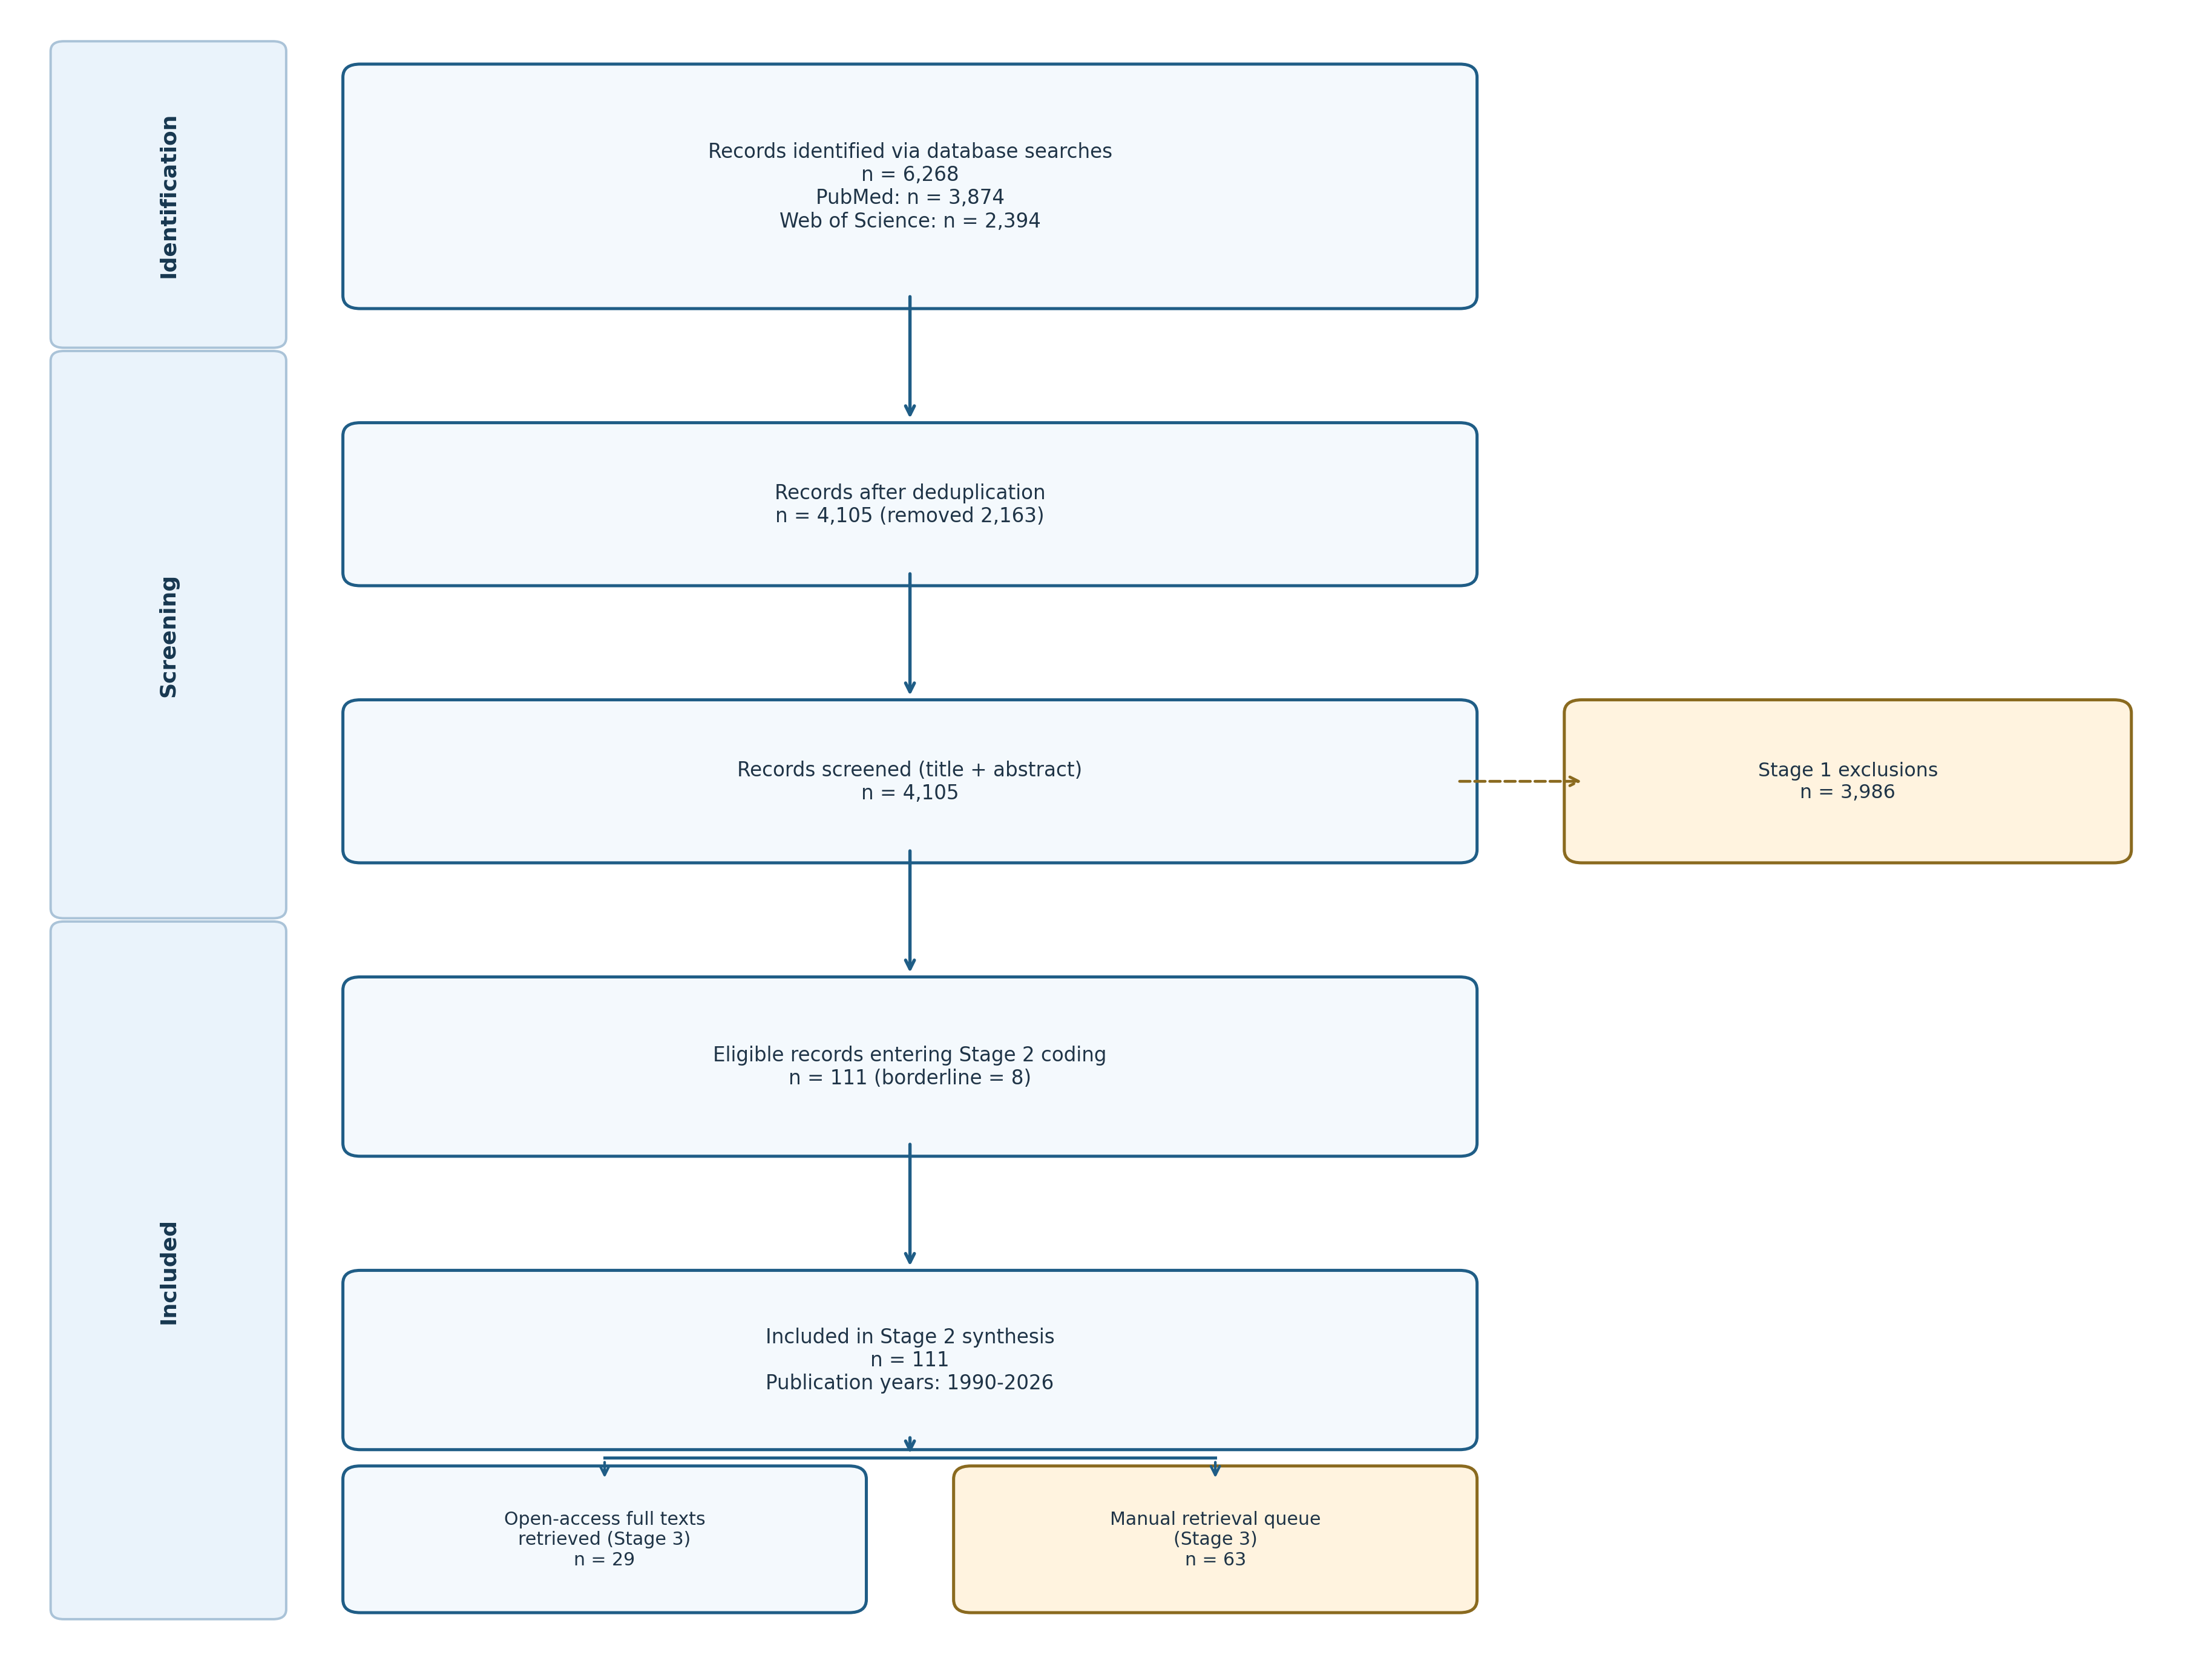
\includegraphics[width=0.94\linewidth,height=0.40\textheight,keepaspectratio]{../assets/figures/prisma_flow.png}
\caption*{\textit{Note.} Three stages: Identification (database searches and deduplication), Screening (title/abstract screening with exclusions), and Included (Stage~2 eligible records and Stage~3 full-text planning). The workflow reflects the operational run covering January~1977--March~2026.}
\end{minipage}
\par\medskip

\subsection{Temporal and Structural Characteristics of Included Reviews}

The included corpus spanned publication years 1990 to 2026, with a marked acceleration in BPS-invoking review output after 2005. Narrative and expert reviews were the dominant review type (73 of 111; 65.8\%), consistent with the predominantly conceptual and clinical orientation of BPS-invoking pain literature; systematic reviews comprised 27 records (24.3\%), with scoping reviews, meta-analyses, and one network meta-analysis accounting for the remainder. By ICD-11 classification, mixed or unspecified chronic pain was the most prevalent category (43 records; 38.7\%), followed by musculoskeletal pain (36; 32.4\%), headache or orofacial pain (15; 13.5\%), and visceral pain (5; 4.5\%). The remaining 12 records span primary chronic pain, postsurgical, neuropathic, and cancer-related categories. Temporal trends, review-type composition, ICD-11 distribution, and BPS domain coverage are shown in Figure~\ref{fig.descriptive.panel}.

% Auto-generated characteristics table — do not edit manually
\begin{landscape}
\setlength{\LTleft}{0pt}
\setlength{\LTright}{0pt}
\setlength{\LTcapwidth}{\linewidth}
\captionsetup{justification=raggedright,singlelinecheck=false}
\setlength{\tabcolsep}{2.0pt}
\renewcommand{\arraystretch}{1.18}
\hbadness=10000
\hfuzz=20pt
\scriptsize
\begin{longtable}{>{\RaggedRight\arraybackslash\hbadness=10000\hfuzz=20pt}p{2.6cm}>{\RaggedRight\arraybackslash\hbadness=10000\hfuzz=20pt}p{8.1cm}>{\RaggedRight\arraybackslash\hbadness=10000\hfuzz=20pt}p{1.9cm}>{\RaggedRight\arraybackslash\hbadness=10000\hfuzz=20pt}p{2.5cm}>{\RaggedRight\arraybackslash\hbadness=10000\hfuzz=20pt}p{2.0cm}>{\RaggedRight\arraybackslash\hbadness=10000\hfuzz=20pt}p{3.0cm}>{\RaggedRight\arraybackslash\hbadness=10000\hfuzz=20pt}p{1.0cm}>{\RaggedRight\arraybackslash\hbadness=10000\hfuzz=20pt}p{2.4cm}}
  \caption{Characteristics of all 111 included reviews.}
  \label{tab.characteristics}\\
  \toprule
  \textbf{Reference} & \textbf{Description} & \textbf{Type} & \textbf{Pain Condition} & \textbf{Objective} & \textbf{BPS Role} & \textbf{Dom.} & \textbf{Typology} \\
  \midrule
  \endfirsthead
  \toprule
  \textbf{Reference} & \textbf{Description} & \textbf{Type} & \textbf{Pain Condition} & \textbf{Objective} & \textbf{BPS Role} & \textbf{Dom.} & \textbf{Typology} \\
  \midrule
  \endhead
  \midrule
  \multicolumn{8}{r}{\scriptsize\textit{Continued on next page}} \\
  \endfoot
  \bottomrule
  \multicolumn{8}{p{0.98\linewidth}}{\footnotesize\textit{Note.} Type: review-design class (for example, narrative, systematic, meta-analysis, or scoping). Pain Condition: ICD-11-oriented chronic pain grouping inferred at abstract level. Objective: primary objective class (clinical, conceptual, methodological, epidemiological, mixed, or unclear). BPS Role: primary declared functional role of BPS language in the review. Dom.: substantive domain mentions in title/objective/abstract after excluding lexical BPS token matches (B\,=\,biological, P\,=\,psychological, S\,=\,social). Typology: provisional BPS operationalization class from Stage~2 abstract-level coding. Description: concise past-tense one-sentence summary generated from cached full-text objective statements when available; otherwise from objective text, abstract, and finally title fallback. References link to DOI (where available) or PubMed record.} \\
  \endlastfoot
\href{https://pubmed.ncbi.nlm.nih.gov/2094850/}{Hampf (1990)} & This narrative review was focused on a biopsychosocial approach to TMJ pain--or looking for keys in the dark. & Narrative review & Musculoskeletal & Conceptual & Explanatory framework & B, P & Pseudo-BPS \\
\href{https://doi.org/10.1097/00006254-199004000-00003}{Lurie \& Borenstein (1990)} & This narrative review was focused on PMS is probably a group of entities which include various symptoms that occur during the 7 to 10 days before. & Narrative review & Mixed/\allowbreak Unspecified & Conceptual & Explanatory framework & B, P, S & Integrative \\
\href{https://doi.org/10.1016/s0950-3579(05)80126-8}{Waddell (1992)} & This narrative review was focused on biopsychosocial analysis of low back pain. & Narrative review & Musculoskeletal & Unclear & Unclear & --- & Pseudo-BPS \\
\href{https://doi.org/10.1007/BF00433377}{Fordyce (1994)} & This narrative review was focused on pain and suffering: what is the unit?. & Narrative review & Musculoskeletal & Clinical & Explanatory framework & P & Pseudo-BPS \\
\href{https://pubmed.ncbi.nlm.nih.gov/8842824/}{Talo et~al. (1996)} & This narrative review was focused on the biopsychosocial disease consequence model in rehabilitation: model development in the Finnish 'work hardening'. & Narrative review & Musculoskeletal & Methodological & Explanatory framework & S & Pseudo-BPS \\
\href{https://pubmed.ncbi.nlm.nih.gov/8940956/}{Ryder (1996)} & This narrative review was focused on chronic pelvic pain in women may involve more than the gynecologic organ systems. & Narrative review & Visceral & Clinical & Explanatory framework & --- & Pseudo-BPS \\
\href{https://pubmed.ncbi.nlm.nih.gov/9927896/}{Moran et~al. (1998)} & This narrative review was focused on psychiatric problems in chronic facial pain. & Narrative review & Headache/\allowbreak Orofacial & Clinical & Rhetorical label & --- & Rhetorical \\
\href{https://pubmed.ncbi.nlm.nih.gov/10635197/}{Molin (1999)} & This narrative review was focused on from bite to mind: TMD--a personal and literature review. & Narrative review & Headache/\allowbreak Orofacial & Conceptual & Explanatory framework & P, S & Pseudo-BPS \\
\href{https://pubmed.ncbi.nlm.nih.gov/10711057/}{Wells-Federman (1999)} & This narrative review was focused on care of the patient with chronic pain: Part I. & Narrative review & Mixed/\allowbreak Unspecified & Clinical & Organizing principle & B, P, S & Integrative \\
\href{https://doi.org/10.1097/00002508-200006001-00002}{Loeser (2000)} & This narrative review was focused on pain and suffering. & Narrative review & Mixed/\allowbreak Unspecified & Conceptual & Rhetorical label & B & Rhetorical \\
\href{https://doi.org/10.1002/14651858.CD002269}{Karjalainen et~al. (2000)} & This systematic review was focused on biopsychosocial rehabilitation for upper limb repetitive strain injuries in working age adults. & Systematic review & Musculoskeletal & Clinical & Intervention rationale & P, S & Pseudo-BPS \\
\href{https://doi.org/10.1053/berh.2000.0113}{Ferrari (2000)} & This narrative review was focused on the biopsychosocial model--a tool for rheumatologists. & Narrative review & Mixed/\allowbreak Unspecified & Conceptual & Explanatory framework & S & Pseudo-BPS \\
\href{https://pubmed.ncbi.nlm.nih.gov/11858295/}{Wells-Federman (2000)} & This narrative review was focused on care of the patient with chronic pain: part II. & Narrative review & Mixed/\allowbreak Unspecified & Clinical & Intervention rationale & B, P, S & Multifactorial \\
\href{https://doi.org/10.1080/09638280110061744}{Truchon (2001)} & This narrative review was focused on determinants of chronic disability related to low back pain: towards an integrative biopsychosocial model. & Narrative review & Musculoskeletal & Conceptual & Explanatory framework & B, P & Pseudo-BPS \\
\href{https://doi.org/10.1136/emj.19.6.526}{Ferrari (2002)} & This narrative review was focused on prevention of chronic pain after whiplash. & Narrative review & Postsurgical & Clinical & Intervention rationale & S & Pseudo-BPS \\
\href{https://doi.org/10.5694/j.1326-5377.2003.tb05287.x}{Goucke (2003)} & This narrative review was focused on the management of persistent pain. & Narrative review & Mixed/\allowbreak Unspecified & Clinical & Intervention rationale & B, P, S & Multifactorial \\
\href{https://doi.org/10.1016/s1047-9651(03)00034-2}{Victor \& Richeimer (2003)} & This narrative review was focused on psychosocial therapies for neck pain. & Narrative review & Musculoskeletal & Clinical & Explanatory framework & P, S & Pseudo-BPS \\
\href{https://doi.org/10.1093/bmb/ldl008}{Waddell (2006)} & This narrative review was focused on preventing incapacity in people with musculoskeletal disorders. & Narrative review & Musculoskeletal & Conceptual & Explanatory framework & P, S & Pseudo-BPS \\
\href{https://pubmed.ncbi.nlm.nih.gov/17149465/}{Low et~al. (2006)} & This narrative review was focused on back injuries--getting injured workers back to work. & Narrative review & Musculoskeletal & Clinical & Intervention rationale & S & Pseudo-BPS \\
\href{https://doi.org/10.1016/j.berh.2006.10.001}{Bergman (2007)} & This narrative review was focused on management of musculoskeletal pain. & Narrative review & Musculoskeletal & Clinical & Explanatory framework & B, P & Pseudo-BPS \\
\href{https://doi.org/10.1111/j.1526-4610.2006.00716.x}{Nicholson et~al. (2007)} & This narrative review was focused on psychological risk factors in headache. & Narrative review & Headache/\allowbreak Orofacial & Conceptual & Explanatory framework & B, P & Pseudo-BPS \\
\href{https://doi.org/10.1212/01.wnl.0000259085.61898.9e}{Jensen et~al. (2007)} & This meta-analysis was focused on the impact of neuropathic pain on health-related quality of life: review and implications. & Meta-analysis & Musculoskeletal & Mixed & Intervention rationale & B & Pseudo-BPS \\
\href{https://doi.org/10.1037/0033-2909.133.4.581}{Gatchel et~al. (2007)} & This narrative review was focused on the biopsychosocial approach to chronic pain: scientific advances and future directions. & Narrative review & Mixed/\allowbreak Unspecified & Conceptual & Explanatory framework & P, S & Pseudo-BPS \\
\href{https://doi.org/10.1038/ncprheum0680}{Scascighini \& Sprott (2008)} & This narrative review was focused on chronic nonmalignant pain: a challenge for patients and clinicians. & Narrative review & Mixed/\allowbreak Unspecified & Clinical & Intervention rationale & P, S & Pseudo-BPS \\
\href{https://doi.org/10.1002/14651858.CD002269.pub2}{Karjalainen et~al. (2009)} & This systematic review was focused on WITHDRAWN: Biopsychosocial rehabilitation for upper limb repetitive strain injuries in working age adults. & Systematic review & Musculoskeletal & Clinical & Intervention rationale & P, S & Pseudo-BPS \\
\href{https://doi.org/10.1016/j.ncl.2009.01.003}{Buse \& Andrasik (2009)} & This systematic review was focused on behavioral medicine for migraine. & Systematic review & Headache/\allowbreak Orofacial & Clinical & Intervention rationale & B, P, S & Multifactorial \\
\href{https://doi.org/10.1891/1541-6577.23.1.42}{Bay \& Liberzon (2009)} & This narrative review was focused on early stress response: a vulnerability framework for functional impairment following mild traumatic brain injury. & Narrative review & Mixed/\allowbreak Unspecified & Conceptual & Explanatory framework & P & Pseudo-BPS \\
\href{https://doi.org/10.1007/s11916-010-0103-0}{Lee \& Tracey (2010)} & This narrative review was focused on unravelling the mystery of pain, suffering, and relief with brain imaging. & Narrative review & Mixed/\allowbreak Unspecified & Conceptual & Explanatory framework & B & Pseudo-BPS \\
\href{https://doi.org/10.1007/s00296-011-1839-5}{Baeza-Velasco et~al. (2011)} & This narrative review was focused on joint hypermobility syndrome: problems that require psychological intervention. & Narrative review & Musculoskeletal & Clinical & Intervention rationale & P, S & Pseudo-BPS \\
\href{https://doi.org/10.1007/s11916-011-0228-9}{Seshia (2012)} & This narrative review was focused on chronic daily headache in children and adolescents. & Narrative review & Headache/\allowbreak Orofacial & Clinical & Intervention rationale & B, P, S & Multifactorial \\
\href{https://doi.org/10.1097/SPC.0b013e328352124f}{Williams \& Cella (2012)} & This narrative review was focused on medically unexplained symptoms and pain: misunderstanding and myth. & Narrative review & Mixed/\allowbreak Unspecified & Conceptual & Explanatory framework & P, S & Pseudo-BPS \\
\href{https://doi.org/10.1179/crn.2012.003}{Simmons (2012)} & This meta-analysis was focused on a critical review of Dr. & Meta-analysis & Headache/\allowbreak Orofacial & Conceptual & Rhetorical label & P, S & Rhetorical \\
\href{https://doi.org/10.1586/ern.12.40}{Renton et~al. (2012)} & This narrative review was focused on the classification and differential diagnosis of orofacial pain. & Narrative review & Headache/\allowbreak Orofacial & Mixed & Justification & B, S & Pseudo-BPS \\
\href{https://doi.org/10.1016/j.ptsp.2011.12.001}{Puentedura \& Louw (2012)} & This systematic review was focused on a neuroscience approach to managing athletes with low back pain. & Systematic review & Musculoskeletal & Clinical & Intervention rationale & B & Pseudo-BPS \\
\href{https://doi.org/10.1016/j.berh.2012.08.004}{Wilkie \& Pransky (2012)} & This narrative review was focused on improving work participation for adults with musculoskeletal conditions. & Narrative review & Musculoskeletal & Clinical & Intervention rationale & B, S & Pseudo-BPS \\
\href{https://doi.org/10.1097/SPC.0b013e32835d7ed2}{Woo et~al. (2013)} & This narrative review was focused on evidence-based approach to manage persistent wound-related pain. & Narrative review & Mixed/\allowbreak Unspecified & Clinical & Intervention rationale & B, P & Pseudo-BPS \\
\href{https://doi.org/10.1185/03007995.2013.810615}{Pergolizzi et~al. (2013)} & This narrative review was focused on the development of chronic pain: physiological CHANGE necessitates a multidisciplinary approach to treatment. & Narrative review & Mixed/\allowbreak Unspecified & Clinical & Intervention rationale & B, P & Pseudo-BPS \\
\href{https://doi.org/10.1097/MOU.0b013e3283652af1}{Williams (2013)} & This narrative review was focused on the importance of psychological assessment in chronic pain. & Narrative review & Mixed/\allowbreak Unspecified & Conceptual & Explanatory framework & B, P & Pseudo-BPS \\
\href{https://doi.org/10.1038/sj.bdj.2013.950}{Durham (2013)} & This narrative review was focused on oral surgery: part 3. & Narrative review & Headache/\allowbreak Orofacial & Clinical & Rhetorical label & --- & Rhetorical \\
\href{https://doi.org/10.1111/head.12272}{Shephard et~al. (2014)} & This narrative review was focused on orofacial pain: a guide for the headache physician. & Narrative review & Headache/\allowbreak Orofacial & Clinical & Intervention rationale & P, S & Pseudo-BPS \\
\href{https://doi.org/10.1186/1471-2474-15-10}{Phyomaung et~al. (2014)} & This systematic review was focused on are depression, anxiety and poor mental health risk factors for knee pain?. & Systematic review & Musculoskeletal & Epidemiological & Intervention rationale & P & Pseudo-BPS \\
\href{https://doi.org/10.1016/j.pmn.2012.08.008}{Matteliano et~al. (2014)} & This systematic review was focused on adherence monitoring with chronic opioid therapy for persistent pain: a biopsychosocial-spiritual approach to. & Systematic review & Mixed/\allowbreak Unspecified & Clinical & Organizing principle & B, P & Pseudo-BPS \\
\href{https://doi.org/10.1097/SPC.0000000000000046}{Novy \& Aigner (2014)} & This narrative review was focused on the biopsychosocial model in cancer pain. & Narrative review & Cancer-related & Conceptual & Explanatory framework & P, S & Pseudo-BPS \\
\href{https://doi.org/10.3928/00904481-20140325-08}{Chogle et~al. (2014)} & This narrative review was focused on pediatric IBS: an overview on pathophysiology, diagnosis and treatment. & Narrative review & Visceral & Conceptual & Explanatory framework & B, P, S & Integrative \\
\href{https://doi.org/10.2147/JPR.S59144}{Gerdle et~al. (2014)} & This narrative review was focused on chronic musculoskeletal pain: review of mechanisms and biochemical biomarkers as assessed by the microdialysis technique. & Narrative review & Musculoskeletal & Conceptual & Explanatory framework & B, P, S & Integrative \\
\href{https://doi.org/10.1016/j.berh.2015.04.005}{Hague \& Shenker (2014)} & This narrative review was focused on how to investigate: Chronic pain. & Narrative review & Mixed/\allowbreak Unspecified & Clinical & Rhetorical label & P, S & Rhetorical \\
\href{https://doi.org/10.2522/ptj.20140575}{Pelletier et~al. (2015)} & This systematic review was focused on addressing Neuroplastic Changes in Distributed Areas of the Nervous System Associated With Chronic Musculoskeletal. & Systematic review & Musculoskeletal & Clinical & Explanatory framework & B, P, S & Integrative \\
\href{https://doi.org/10.3390/bs5020264}{Kent et~al. (2015)} & This narrative review was focused on goal-Directed Resilience in Training (GRIT): A Biopsychosocial Model of Self-Regulation, Executive Functions, and. & Narrative review & Mixed/\allowbreak Unspecified & Clinical & Intervention rationale & B, P & Pseudo-BPS \\
\href{https://doi.org/10.1177/1756285615605699}{Obermann et~al. (2015)} & This narrative review was focused on an update on the management of post-traumatic headache. & Narrative review & Postsurgical & Clinical & Intervention rationale & P, S & Pseudo-BPS \\
\href{https://doi.org/10.1111/ajd.12365}{Thornton \& Drummond (2016)} & This narrative review was focused on current concepts in vulvodynia with a focus on pathogenesis and pain mechanisms. & Narrative review & Primary & Clinical & Intervention rationale & B, P, S & Multifactorial \\
\href{https://doi.org/10.1016/j.mcna.2015.09.005}{Walk \& Poliak-Tunis (2016)} & This narrative review was focused on chronic Pain Management: An Overview of Taxonomy, Conditions Commonly Encountered, and Assessment. & Narrative review & Mixed/\allowbreak Unspecified & Clinical & Organizing principle & P & Pseudo-BPS \\
\href{https://doi.org/10.1016/j.mcna.2015.08.007}{Cheatle (2016)} & This narrative review was focused on biopsychosocial Approach to Assessing and Managing Patients with Chronic Pain. & Narrative review & Mixed/\allowbreak Unspecified & Clinical & Intervention rationale & P & Pseudo-BPS \\
\href{https://doi.org/10.1097/AJP.0000000000000342}{Giummarra et~al. (2016)} & This systematic review was focused on chronic Pain Following Motor Vehicle Collision: A Systematic Review of Outcomes Associated With Seeking or Receiving. & Systematic review & Postsurgical & Epidemiological & Explanatory framework & P, S & Pseudo-BPS \\
\href{https://doi.org/10.1097/j.pain.0000000000000572}{Ditre et~al. (2016)} & This meta-analysis was focused on acute analgesic effects of nicotine and tobacco in humans. & Meta-analysis & Mixed/\allowbreak Unspecified & Epidemiological & Rhetorical label & --- & Rhetorical \\
\href{https://doi.org/10.1016/j.neubiorev.2016.05.033}{Borsook et~al. (2016)} & This systematic review was focused on reward deficiency and anti-reward in pain chronification. & Systematic review & Mixed/\allowbreak Unspecified & Conceptual & Explanatory framework & P & Pseudo-BPS \\
\href{https://doi.org/10.1016/j.nec.2016.02.012}{Zakrzewska (2016)} & This systematic review was focused on chronic/Persistent Idiopathic Facial Pain. & Systematic review & Headache/\allowbreak Orofacial & Clinical & Intervention rationale & P & Pseudo-BPS \\
\href{https://doi.org/10.1016/j.mayocp.2016.04.029}{Hooten (2016)} & This narrative review was focused on chronic Pain and Mental Health Disorders: Shared Neural Mechanisms, Epidemiology, and Treatment. & Narrative review & Mixed/\allowbreak Unspecified & Clinical & Explanatory framework & B, P & Pseudo-BPS \\
\href{https://doi.org/10.1080/09593985.2016.1194651}{Wijma et~al. (2016)} & This narrative review was focused on clinical biopsychosocial physiotherapy assessment of patients with chronic pain: The first step in pain neuroscience. & Narrative review & Mixed/\allowbreak Unspecified & Clinical & Organizing principle & B, P, S & Integrative \\
\href{https://doi.org/10.1097/MOH.0000000000000282}{Robinson \& Fuchs (2016)} & This narrative review was focused on allogeneic stem cell transplantation for sickle cell disease. & Narrative review & Mixed/\allowbreak Unspecified & Clinical & Rhetorical label & --- & Rhetorical \\
\href{https://doi.org/10.1097/j.pain.0000000000000775}{Fillingim (2017)} & This narrative review was focused on individual differences in pain: understanding the mosaic that makes pain personal. & Narrative review & Mixed/\allowbreak Unspecified & Conceptual & Explanatory framework & B, P & Pseudo-BPS \\
\href{https://doi.org/10.5694/mja16.00828}{Bardin et~al. (2017)} & This narrative review was focused on diagnostic triage for low back pain: a practical approach for primary care. & Narrative review & Musculoskeletal & Clinical & Organizing principle & --- & Pseudo-BPS \\
\href{https://doi.org/10.1002/msc.1191}{Booth et~al. (2017)} & This narrative review was focused on exercise for chronic musculoskeletal pain: A biopsychosocial approach. & Narrative review & Musculoskeletal & Clinical & Intervention rationale & B, P, S & Multifactorial \\
\href{https://doi.org/10.1007/s11926-017-0683-3}{Bartley et~al. (2017)} & This systematic review was focused on predictors of Osteoarthritis Pain: the Importance of Resilience. & Systematic review & Musculoskeletal & Conceptual & Explanatory framework & S & Pseudo-BPS \\
\href{https://doi.org/10.1016/j.ijosm.2018.07.001}{Draper-Rodi et~al. (2018)} & This scoping review was focused on identification of prognostic factors and assessment methods on the evaluation of non-specific low back pain in a. & Scoping review & Musculoskeletal & Clinical & Organizing principle & --- & Pseudo-BPS \\
\href{https://doi.org/10.1016/j.pnpbp.2017.09.022}{Gagliese et~al. (2018)} & This systematic review was focused on pain, aging and dementia: Towards a biopsychosocial model. & Systematic review & Mixed/\allowbreak Unspecified & Conceptual & Explanatory framework & B, P & Pseudo-BPS \\
\href{https://doi.org/10.1007/s00586-017-5433-8}{Chou et~al. (2018)} & This systematic review was focused on the Global Spine Care Initiative: applying evidence-based guidelines on the non-invasive management of back and neck. & Systematic review & Musculoskeletal & Clinical & Intervention rationale & B, P, S & Multifactorial \\
\href{https://doi.org/10.1097/ALN.0000000000002137}{Martucci \& Mackey (2018)} & This narrative review was focused on neuroimaging of Pain: Human Evidence and Clinical Relevance of Central Nervous System Processes and Modulation. & Narrative review & Mixed/\allowbreak Unspecified & Conceptual & Rhetorical label & B, S & Rhetorical \\
\href{https://doi.org/10.1111/papr.12706}{Tai et~al. (2018)} & This systematic review was focused on enriched Environment and Effects on Neuropathic Pain: Experimental Findings and Mechanisms. & Systematic review & Neuropathic & Clinical & Rhetorical label & B, P & Rhetorical \\
\href{https://doi.org/10.1016/j.hoc.2018.01.014}{Brandow \& DeBaun (2018)} & This narrative review was focused on key Components of Pain Management for Children and Adults with Sickle Cell Disease. & Narrative review & Mixed/\allowbreak Unspecified & Clinical & Background framing & B & Rhetorical \\
\href{https://doi.org/10.1097/ACO.0000000000000675}{Luchting \& Azad (2019)} & This narrative review was focused on pain therapy for the elderly patient: is opioid-free an option?. & Narrative review & Mixed/\allowbreak Unspecified & Clinical & Intervention rationale & B, P & Pseudo-BPS \\
\href{https://doi.org/10.1016/j.clinbiomech.2018.12.010}{Mousavi et~al. (2019)} & This narrative review was focused on low back pain: Moving toward mechanism-based management. & Narrative review & Musculoskeletal & Clinical & Intervention rationale & --- & Pseudo-BPS \\
\href{https://doi.org/10.1097/SPC.0000000000000420}{Schweinhardt (2019)} & This narrative review was focused on where has the 'bio' in bio-psycho-social gone?. & Narrative review & Postsurgical & Conceptual & Explanatory framework & B, P & Pseudo-BPS \\
\href{https://doi.org/10.3390/jcm8091334}{Ford et~al. (2019)} & This narrative review was focused on the Evolving Case Supporting Individualised Physiotherapy for Low Back Pain. & Narrative review & Musculoskeletal & Clinical & Intervention rationale & --- & Pseudo-BPS \\
\href{https://doi.org/10.3390/medicina56010006}{Paley \& Johnson (2019)} & This systematic review was focused on acupuncture for the Relief of Chronic Pain: A Synthesis of Systematic Reviews. & Systematic review & Mixed/\allowbreak Unspecified & Clinical & Background framing & B, P, S & Multifactorial \\
\href{https://doi.org/10.5606/ArchRheumatol.2019.6801}{Şen et~al. (2019)} & This systematic review was focused on group Psychotherapy With Fibromyalgia Patients. & Systematic review & Primary & Clinical & Conclusion & P, S & Rhetorical \\
\href{https://doi.org/10.1097/j.pain.0000000000001809}{Holopainen et~al. (2020)} & This systematic review was focused on physiotherapists' perceptions of learning and implementing a biopsychosocial intervention to treat musculoskeletal. & Systematic review & Musculoskeletal & Clinical & Intervention rationale & --- & Pseudo-BPS \\
\href{https://doi.org/10.11607/ofph.2608}{Greene \& Manfredini (2020)} & This narrative review was focused on treating Temporomandibular Disorders in the 21st Century: Can We Finally Eliminate the "Third Pathway"?. & Narrative review & Headache/\allowbreak Orofacial & Clinical & Justification & S & Pseudo-BPS \\
\href{https://doi.org/10.1097/MD.0000000000021969}{Nduwimana et~al. (2020)} & This meta-analysis was focused on effectiveness of walking versus mind-body therapies in chronic low back pain: A systematic review and meta-analysis. & Meta-analysis & Musculoskeletal & Clinical & Intervention rationale & --- & Pseudo-BPS \\
\href{https://doi.org/10.1071/HC19117}{Baxter et~al. (2020)} & This narrative review was focused on six things you need to know about low back pain. & Narrative review & Musculoskeletal & Clinical & Intervention rationale & --- & Pseudo-BPS \\
\href{https://doi.org/10.3390/ijerph18010246}{D'Amico et~al. (2020)} & This scoping review was focused on mapping Assessments Instruments for Headache Disorders against the ICF Biopsychosocial Model of Health and Disability. & Scoping review & Headache/\allowbreak Orofacial & Methodological & Organizing principle & P, S & Pseudo-BPS \\
\href{https://doi.org/10.1016/j.anclin.2020.11.004}{Xu et~al. (2021)} & This narrative review was focused on pain Management in Neurosurgery: Back and Lower Extremity Pain, Trigeminal Neuralgia. & Narrative review & Mixed/\allowbreak Unspecified & Clinical & Intervention rationale & --- & Pseudo-BPS \\
\href{https://doi.org/10.1080/14737175.2021.1900734}{Argyriou et~al. (2021)} & This systematic review was focused on an updated brief overview on post-traumatic headache and a systematic review of the non-pharmacological. & Systematic review & Headache/\allowbreak Orofacial & Clinical & Intervention rationale & B, P, S & Multifactorial \\
\href{https://pubmed.ncbi.nlm.nih.gov/34793635/}{Najem et~al. (2021)} & This systematic review was focused on religious Beliefs and Attitudes in Relation to Pain, Pain-Related Beliefs, Function, and Coping in Chronic. & Systematic review & Musculoskeletal & Clinical & Background framing & P & Rhetorical \\
\href{https://doi.org/10.1007/164_2022_587}{Mustafa et~al. (2022)} & This narrative review was focused on toll-Like Receptor 4 in Pain: Bridging Molecules-to-Cells-to-Systems. & Narrative review & Mixed/\allowbreak Unspecified & Conceptual & Explanatory framework & B, P & Pseudo-BPS \\
\href{https://doi.org/10.1097/GRF.0000000000000712}{Green et~al. (2022)} & This narrative review was focused on persistent Pelvic Pain in Patients With Endometriosis. & Narrative review & Visceral & Clinical & Organizing principle & B & Pseudo-BPS \\
\href{https://doi.org/10.1136/bmjsem-2022-001326}{Edgar et~al. (2022)} & This narrative review was focused on biopsychosocial approach to tendinopathy. & Narrative review & Musculoskeletal & Clinical & Intervention rationale & B, P, S & Multifactorial \\
\href{https://doi.org/10.3390/jfmk7040074}{Ferlito et~al. (2022)} & This systematic review was focused on pain Education in the Management of Patients with Chronic Low Back Pain. & Systematic review & Musculoskeletal & Clinical & Intervention rationale & P, S & Pseudo-BPS \\
\href{https://doi.org/10.3390/jcm12237489}{Jurak et~al. (2023)} & This network meta-analysis was focused on effects of Multidisciplinary Biopsychosocial Rehabilitation on Short-Term Pain and Disability in Chronic Low Back. & Network meta-analysis & Musculoskeletal & Clinical & Intervention rationale & --- & Pseudo-BPS \\
\href{https://doi.org/10.1080/09593985.2022.2080130}{Cormack et~al. (2023)} & This narrative review was focused on the biopsychosocial model is lost in translation: from misrepresentation to an enactive modernization. & Narrative review & Musculoskeletal & Conceptual & Explanatory framework & S & Pseudo-BPS \\
\href{https://doi.org/10.1007/s11916-022-01098-8}{Overstreet et~al. (2023)} & This narrative review was focused on the Experience of BIPOC Living with Chronic Pain in the USA: Biopsychosocial Factors that Underlie Racial. & Narrative review & Mixed/\allowbreak Unspecified & Epidemiological & Explanatory framework & B, P, S & Integrative \\
\href{https://doi.org/10.3390/jcm12020526}{Włodarczyk et~al. (2023)} & This narrative review was focused on management of Pelvic Pain in Patients with Crohn's Disease-Current Overview. & Narrative review & Visceral & Clinical & Background framing & B & Rhetorical \\
\href{https://doi.org/10.1089/jpm.2022.0571}{Gerhart et~al. (2023)} & This narrative review was focused on top Ten Tips Palliative Care Clinicians Should Know About Behavioral Pain Management for Persistent Pain. & Narrative review & Mixed/\allowbreak Unspecified & Clinical & Explanatory framework & P & Pseudo-BPS \\
\href{https://doi.org/10.14309/ajg.0000000000002216}{Frazier et~al. (2023)} & This narrative review was focused on diagnosis and Management of Cyclic Vomiting Syndrome: A Critical Review. & Narrative review & Headache/\allowbreak Orofacial & Clinical & Intervention rationale & B, P, S & Multifactorial \\
\href{https://doi.org/10.1055/s-0043-1770715}{Carey \& McClurg (2023)} & This systematic review was focused on evaluation and Medical Management of Chronic Pelvic Pain. & Systematic review & Visceral & Clinical & Intervention rationale & --- & Pseudo-BPS \\
\href{https://doi.org/10.3390/diagnostics13243689}{Rahman et~al. (2023)} & This narrative review was focused on clinical Diagnosis and Treatment of Chronic Pain. & Narrative review & Mixed/\allowbreak Unspecified & Clinical & Organizing principle & --- & Pseudo-BPS \\
\href{https://doi.org/10.3390/biomedicines11123174}{Ruimonte-Crespo et~al. (2023)} & This narrative review was focused on aerobic Exercise and Neuropathic Pain: Insights from Animal Models and Implications for Human Therapy. & Narrative review & Neuropathic & Clinical & Rhetorical label & B & Rhetorical \\
\href{https://doi.org/10.1007/s00406-023-01721-8}{Shil et~al. (2024)} & This narrative review was focused on a clinical approach to the investigation and management of long COVID associated neuropathic pain. & Narrative review & Neuropathic & Clinical & Intervention rationale & B & Pseudo-BPS \\
\href{https://doi.org/10.3390/healthcare12050575}{Warzocha et~al. (2024)} & This systematic review was focused on etiologic Factors of Temporomandibular Disorders: A Systematic Review of Literature Containing Diagnostic Criteria. & Systematic review & Headache/\allowbreak Orofacial & Epidemiological & Rhetorical label & P, S & Rhetorical \\
\href{https://doi.org/10.26635/6965.6513}{Polonowita et~al. (2024)} & This narrative review was focused on construction of the chronic temporomandibular disorder patients: the association between neural and psychological. & Narrative review & Mixed/\allowbreak Unspecified & Conceptual & Explanatory framework & B, P, S & Integrative \\
\href{https://doi.org/10.1371/journal.pone.0308625}{Lawan et~al. (2024)} & This meta-analysis was focused on is educational attainment associated with the onset and outcomes of low back pain?. & Meta-analysis & Musculoskeletal & Methodological & Unclear & S & Pseudo-BPS \\
\href{https://doi.org/10.1186/s41927-024-00430-6}{Couëpel et~al. (2024)} & This scoping review was focused on what are the functional and clinical characteristics shared by fibromyalgia and low back pain?. & Scoping review & Primary & Clinical & Organizing principle & B, P, S & Integrative \\
\href{https://doi.org/10.3389/fmolb.2024.1382555}{Dehghan et~al. (2024)} & This narrative review was focused on deciphering pain: molecular mechanisms and neurochemical pathways-challenges and future opportunities. & Narrative review & Mixed/\allowbreak Unspecified & Conceptual & Explanatory framework & B & Pseudo-BPS \\
\href{https://doi.org/10.3390/medicina60122065}{Alonso-Sal et~al. (2024)} & This systematic review was focused on effectiveness of Physical Activity in the Management of Nonspecific Low Back Pain. & Systematic review & Musculoskeletal & Clinical & Intervention rationale & B, P & Pseudo-BPS \\
\href{https://doi.org/10.1097/j.pain.0000000000003406}{Rometsch et~al. (2025)} & This systematic review was focused on chronic pain in European adult populations: a systematic review of prevalence and associated clinical features. & Systematic review & Mixed/\allowbreak Unspecified & Epidemiological & Background framing & P, S & Rhetorical \\
\href{https://doi.org/10.1002/ejp.70016}{Souza et~al. (2025)} & This scoping review was focused on conversational Agents to Support Pain Management. & Scoping review & Mixed/\allowbreak Unspecified & Clinical & Background framing & P & Rhetorical \\
\href{https://doi.org/10.1093/joccuh/uiaf028}{Kubala et~al. (2025)} & This systematic review was focused on biopsychosocial and physical factors associated with firefighter musculoskeletal disorders. & Systematic review & Musculoskeletal & Epidemiological & Organizing principle & P, S & Pseudo-BPS \\
\href{https://doi.org/10.1186/s12939-025-02560-w}{Potthoff et~al. (2025)} & This systematic review was focused on social dimensions as explanatory approaches for the development of chronic pain: a meta-ethnography of qualitative. & Systematic review & Mixed/\allowbreak Unspecified & Conceptual & Explanatory framework & B, P, S & Integrative \\
\href{https://doi.org/10.1016/j.ncl.2025.04.005}{Mueller et~al. (2025)} & This systematic review was focused on advances in Our Understanding and Treatment of Nociplastic Pain. & Systematic review & Primary & Clinical & Intervention rationale & B & Pseudo-BPS \\
\href{https://doi.org/10.1111/ejn.70275}{Strien \& Hollmann (2025)} & This narrative review was focused on pain Perception and Modulation: Fundamental Neurobiology and Recent Advances. & Narrative review & Mixed/\allowbreak Unspecified & Conceptual & Explanatory framework & B, P & Pseudo-BPS \\
\href{https://doi.org/10.1111/aphw.70093}{Kohlert et~al. (2025)} & This scoping review was focused on existential therapy for treating chronic pain. & Scoping review & Mixed/\allowbreak Unspecified & Clinical & Intervention rationale & P & Pseudo-BPS \\
\href{https://doi.org/10.1016/j.cger.2025.08.005}{Boon et~al. (2026)} & This narrative review was focused on dual Experience and Management of Pain in Older Adults and Their Caregivers. & Narrative review & Mixed/\allowbreak Unspecified & Clinical & Explanatory framework & S & Pseudo-BPS \\
\end{longtable}
\renewcommand{\arraystretch}{1}
\normalsize
\end{landscape}


\begin{figure}[!ht]
  \caption{Descriptive structure of the included evidence base across four dimensions.}
  \label{fig.descriptive.panel}
  \centering
  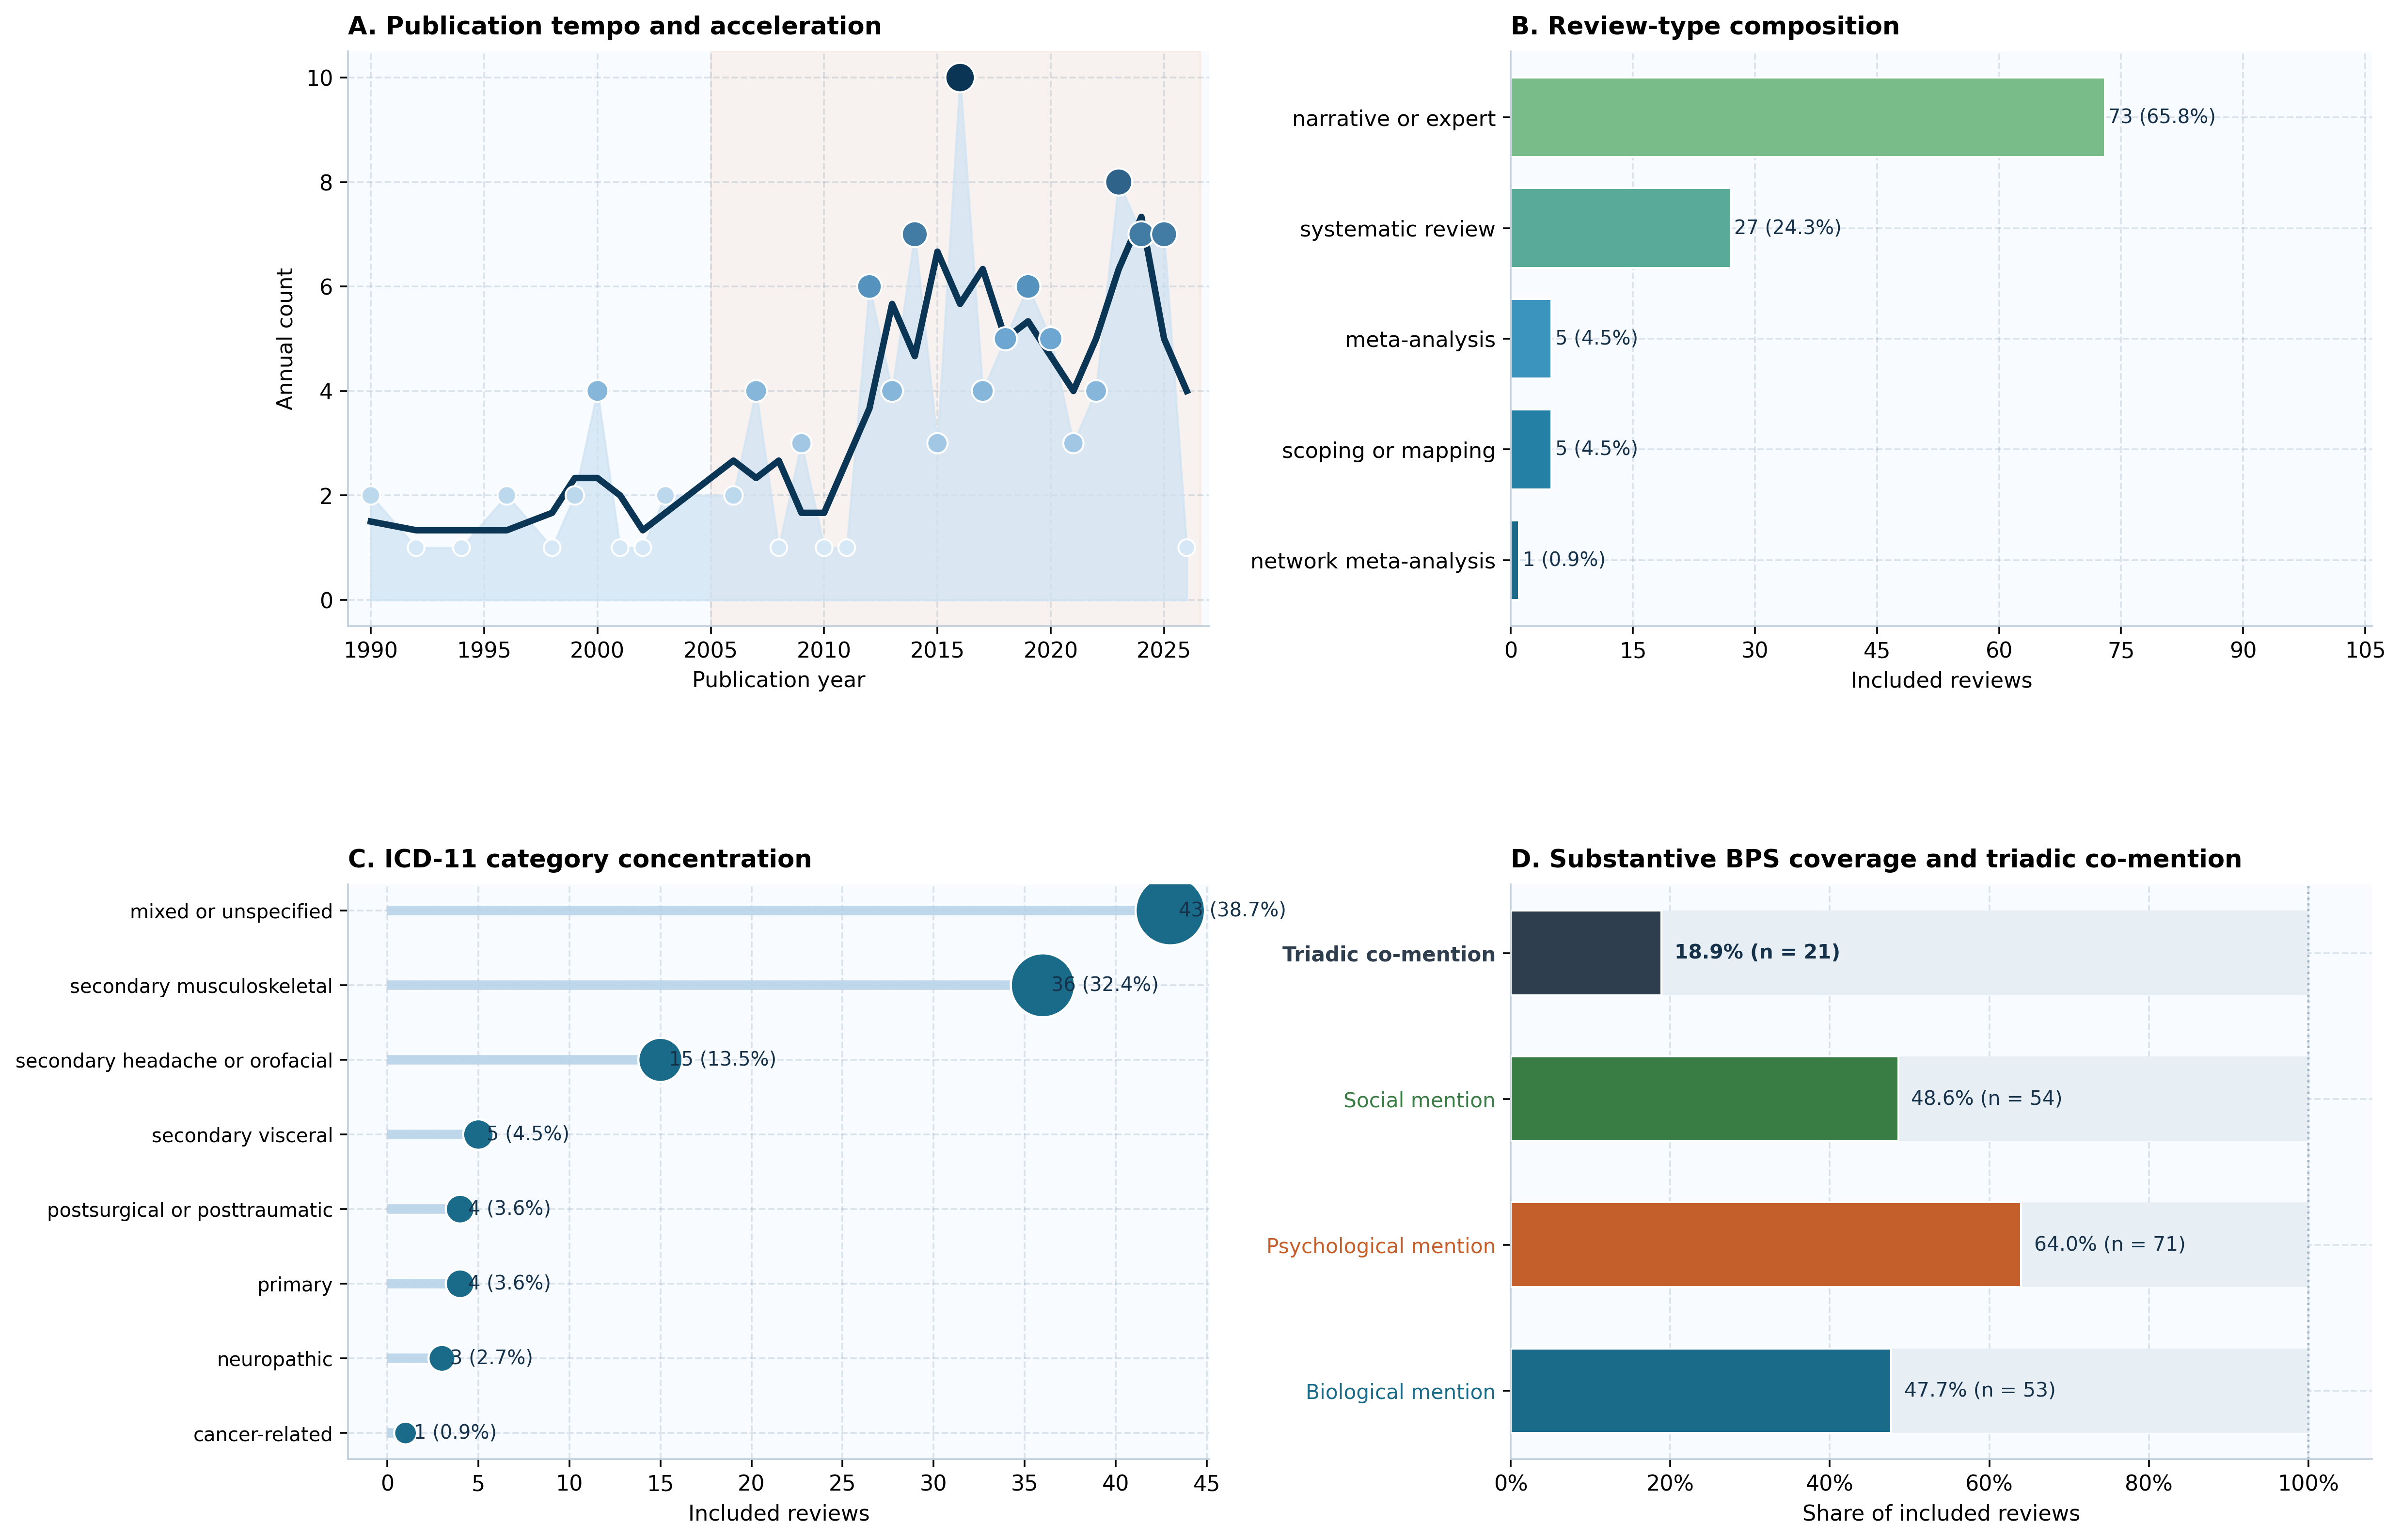
\includegraphics[width=0.98\textwidth]{../assets/figures/descriptive_panel_abcd.png}
  \caption*{\textit{Note.} Panel~A shows annual publication counts ($n = 111$) with a 3-year rolling trend line and post-2005 growth shading. Panel~B shows review-type distribution with frequency labels. Panel~C shows concentration across ICD-11 categories. Panel~D compares biological, psychological, and social substantive-domain coverage plus overall triadic co-mention frequency across all 111 records.}
\end{figure}

\subsection{Biopsychosocial Operationalization}
\label{subsec:rq1}

\subsubsection*{Mention Location and Functional Role}

BPS terminology appeared predominantly in the abstract without title mention in 87 records (78.4\%), indicating that for most reviews the model functions as methodological or conceptual context rather than as the primary subject of inquiry. A further 18 records (16.2\%) mentioned BPS in both title and abstract, and 6 (5.4\%) in the title only. The most common declared functional role was intervention rationale (41 records; 36.9\%), followed by explanatory framework (37; 33.3\%), organizing principle (11; 9.9\%), rhetorical label (11; 9.9\%), and background framing (6; 5.4\%). Many records using the explanatory framework label do not provide mechanistic elaboration of domain interactions, providing partial support for study hypothesis H4.

\subsubsection*{Provisional Typological Classification}

The provisional typological scheme identified pseudo-BPS or partial signal as the dominant category (73 records; 65.8\%), followed by rhetorical label signal (17; 15.3\%), multifactorial signal (11; 9.9\%), and potential integrative signal (10; 9.0\%). Thus, approximately four in five records fall below the potential-integrative threshold at abstract level. These typological estimates are provisional pending Stage~3 full-text adjudication and address study hypotheses H1 and H2. Figure~\ref{fig.operationalization.combined} (Panel~A) visualizes the distribution; Panel~B shows the cross-tabulation of BPS function by objective category.

\begin{figure}[htbp]
  \caption{Biopsychosocial operationalization structure: typology, BPS function, musculoskeletal domain coverage, and full-corpus domain mentions.}
  \label{fig.operationalization.combined}
  \centering
  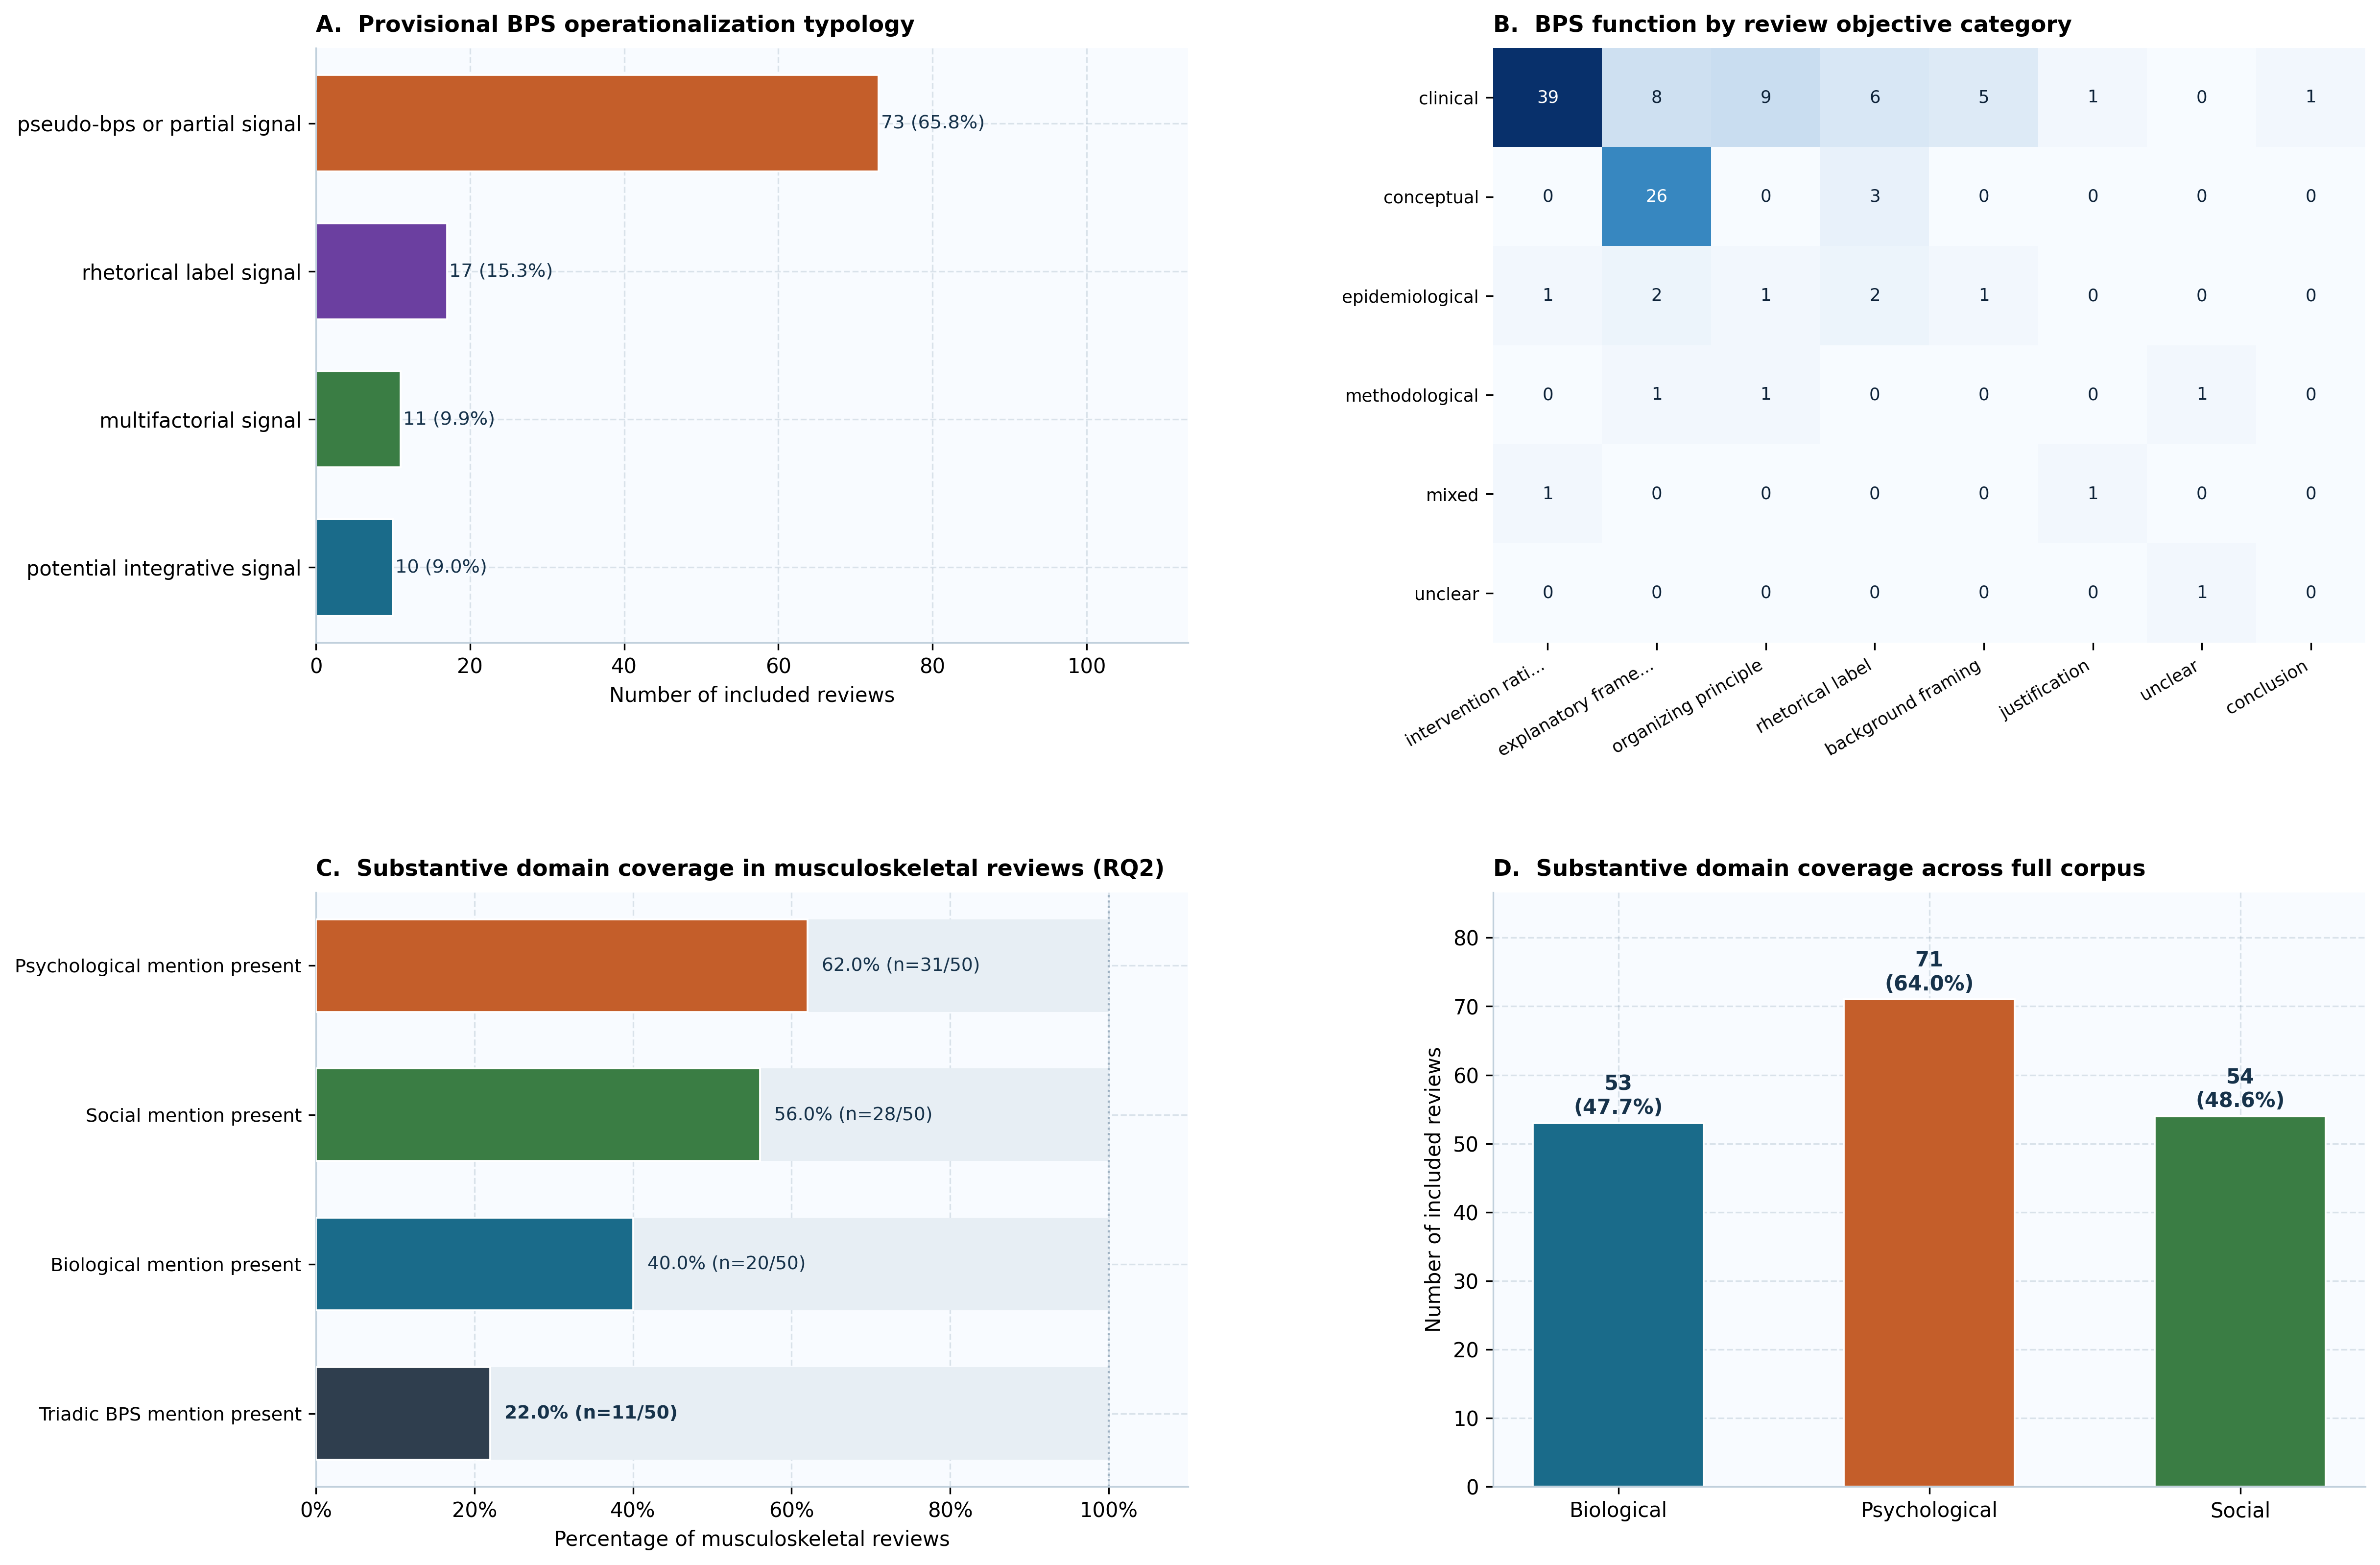
\includegraphics[width=0.99\textwidth]{../assets/figures/operationalization_combined.png}
  \caption*{\textit{Note.} Panel~A: provisional typological distribution (RQ1); categories are assigned by Stage~2 coding and remain provisional pending Stage~3 adjudication. Panel~B: cross-tabulation of BPS functional role by objective category; cell values are record counts. Panel~C: substantive-domain coverage within the 50 musculoskeletal reviews (RQ2); bars show percentage of musculoskeletal records with each domain/triadic mention. Panel~D: overall biological, psychological, and social substantive-domain frequencies across all 111 included records.}
\end{figure}

\noindent\textbf{BPS Operationalization.} Across 111 included reviews, BPS terminology appeared predominantly in the abstract without title mention (dominant location: abstract only; 87 records, 78.4\%). The most common declared functional role was \textit{intervention rationale} (36.9\%), followed by explanatory framework (33.3\%), together accounting for 70.2\% of the corpus. Provisional typological classification: potential integrative signal 9.0\%, multifactorial signal 9.9\%, pseudo-BPS or partial signal 65.8\%, rhetorical label signal 9.9\%. This distribution provides empirical support for the pre-specified hypothesis that BPS language is often used as a rhetorical or contextualizing device rather than as a specification of triadic mechanistic integration. Evidence is visualized in Figure~\ref{fig.operationalization.combined} (Panels~A and~B).

\par\medskip
\noindent\textbf{Scope, Balance, and Integration in Musculoskeletal Reviews.} Using the substantive domain-coding layer (lexical BPS token matches excluded), coverage within the 50 musculoskeletal reviews was: biological 20/50 (40.0\%), psychological 31/50 (62.0\%), social 28/50 (56.0\%). Simultaneous triadic co-mention was present in 11/50 musculoskeletal reviews (22.0\%). Across all 111 Stage~2 records, triadic co-mention was 21/111 (18.9\%). Ontology-aligned semantic loading (covering 111 records) identified psychological orientation as dominant in 52 records (46.8\%), biological in 48 (43.2\%), and social in 11 (9.9\%). Mean domain loadings were: biological 0.341, psychological 0.341, social 0.318. Taken together, the two layers indicate divergence between domain naming and semantic weight: social content is often present but comparatively light in semantic centrality. Evidence is in Figure~\ref{fig.operationalization.combined} (Panels~C and~D), Figure~\ref{fig.semantic.loading.combined}, and Figure~\ref{fig.semantic.landscape.integrated}.

\par\medskip
\noindent\textbf{Psychological Concepts and Frameworks.} Across 111 Stage~2 records, 51/111 (45.9\%) contained at least one explicit psychological construct token in abstract-level coding. A total of 95 construct occurrences were detected; ranked frequencies were: depression (22; 23.2\%); stress (19; 20.0\%); anxiety (16; 16.8\%); coping (8; 8.4\%); catastrophizing (4; 4.2\%); fear-avoidance (4; 4.2\%). The top three concepts (depression, stress, anxiety) accounted for 60.0\% of all detected construct occurrences, indicating concentration in high-level affect labels. By contrast, theoretically specific mechanism-oriented constructs (for example, catastrophizing, fear-avoidance, self-efficacy, and illness perception) appeared less frequently, supporting a profile in which symptom-language is more prevalent than explicit mechanism-language at abstract level. Framework mentions were comparatively sparse (9 total mentions); top entries were: neuroscience (2; 22.2\%); mechanistic approach (1; 11.1\%); fear-avoidance model (1; 11.1\%). Ontology-based subdomain loading further indicated that psychological-domain weight is carried primarily by broad cognitive-behavioral and affective clusters rather than narrowly specified mechanistic frameworks. Stage~3 full-text coding will refine construct definitions, framework attribution, and hierarchical mapping under manual adjudication. Evidence is in Figure~\ref{fig.semantic.loading.combined} (Panel~A) and the supplementary semantic tables.


\subsection{Scope, Balance, and Integration in Musculoskeletal Reviews}
\label{subsec:rq2}

Addressing \ref{rq2}, the analysis focused on the 50 reviews classified as chronic secondary musculoskeletal pain.

\subsubsection*{Structured Domain Coverage}

Domain mention frequencies for the musculoskeletal subset are illustrated in Figure~\ref{fig.operationalization.combined} (Panel~C). In the substantive-domain coding layer (which excludes lexical BPS token matches), social factors were present in 28 of 50 reviews (56.0\%), psychological factors in 31 of 50 (62.0\%), and biological factors in 20 of 50 (40.0\%). Triadic mention was present in 11 of 50 musculoskeletal reviews (22.0\%). The musculoskeletal subset therefore shows moderate two-domain coverage but limited explicit triadic integration at abstract level, leaving study hypotheses H2 and H3 partially satisfied at this interim stage.

The domain mention pattern across the full corpus of 111 reviews is illustrated in Figure~\ref{fig.operationalization.combined} (Panel~D). Substantive-domain frequencies were psychological 64.0\%, social 48.6\%, and biological 47.7\%, with triadic co-mention at 18.9\%. The main structural deficit at abstract level is therefore not absence of a single domain, but the recurrent failure to combine all three domains in a clearly articulated integrative logic.

\subsubsection*{Semantic Domain Loading and the Social Deficit}

Ontology-aligned semantic loading provided a continuous, text-derived perspective on domain balance. Across all 111 included records, psychological orientation was semantically dominant in 46.8\% of records, biological in 43.2\%, and social in only 9.9\% (supplementary Table~\ref{tab.semantic.summary} and Figure~\ref{fig.semantic.loading.combined}). Mean domain loadings were: biological~0.341, psychological~0.341, social~0.318. The social loading deficit---despite substantial social naming in structured coding---constitutes a robust signal that social factors remain comparatively underweighted in semantic centrality, consistent with study hypothesis H3 \citep{dorner2011, harkness2005, edwards2016}.

Figure~\ref{fig.semantic.loading.combined} (Panel~A) shows the two-layer domain hierarchy: the inner ring presents domain-level loading proportions and the right panel resolves each domain into its 42 ontology subdomains with within-domain normalized loading bars. Within the biological domain, pharmacological/biomedical treatment and central sensitization subdomains carry the highest relative loading. Within psychology, cognitive-behavioral and third-wave therapy subdomains lead, followed by healthcare-seeking and attention/vigilance constructs. Within social, healthcare access and social determinants subdomains rank highest. Panel~B reframes the semantic-loading result as benchmark-relative deviations: biological and psychological loadings sit slightly above the equal-share benchmark on average, whereas social loading is shifted below it. Thus the key signal is not large dispersion across BPS space but a repeated, corpus-wide social shortfall.

\begin{figure}[!ht]
  \caption{Two-layer ontology semantic loading across the BPS hierarchy and benchmark-relative domain deviation distributions.}
  \label{fig.semantic.loading.combined}
  \centering
  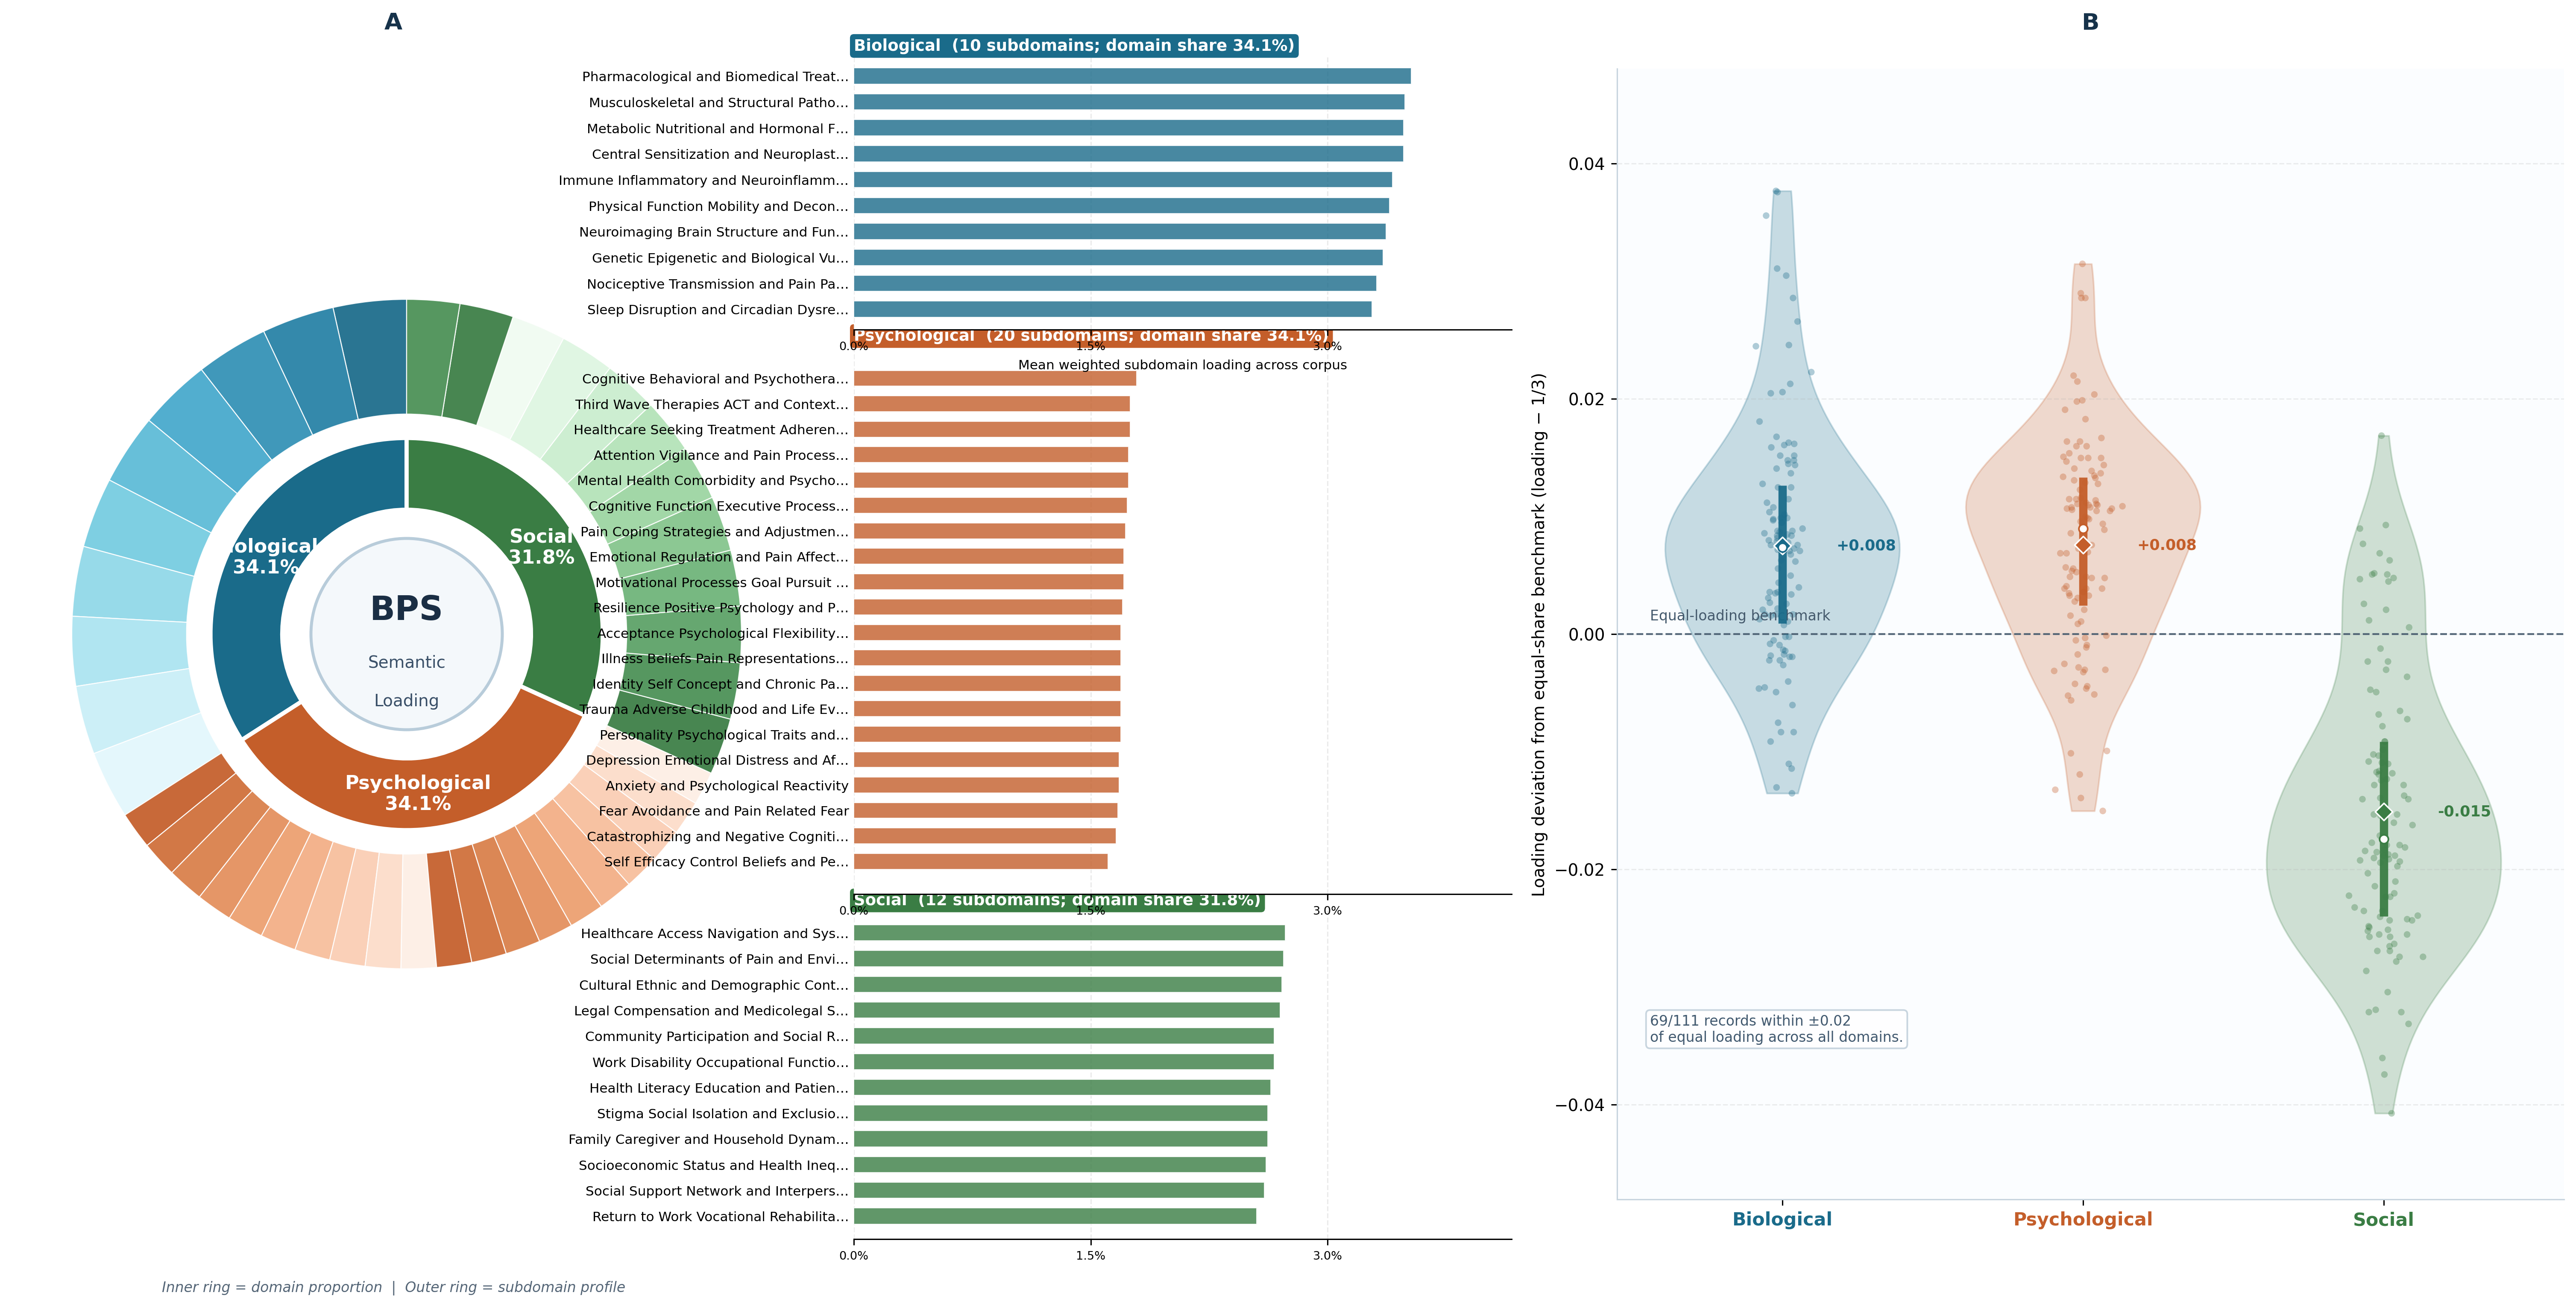
\includegraphics[width=0.99\textwidth]{../assets/figures/semantic_loading_combined.png}

  \caption*{\textit{Note.} Panel~A: left sub-panel shows the two-ring sunburst (inner ring = domain-level loading proportions; outer ring = 42 subdomain segments without text to avoid overlap); right sub-panel shows mean weighted subdomain loading percentages (absolute, not within-domain normalized) grouped by domain, with domain-share labels. Segment and bar magnitudes are proportional to corpus-level mean weighted loading across 111 records. Panel~B: each domain's distribution of deviation from the equal-share benchmark (loading~$-$~1/3), with violin density, raw jittered points, and mean (diamond) and median markers.}
\end{figure}

\subsubsection*{Pairwise and Triadic Co-loading}

Pairwise loading products measure the co-occurrence of two domains within the same semantic space of a record. Figure~\ref{fig.semantic.landscape.integrated} shows that the bio$\times$psychological term is shifted above the equal-balance benchmark, whereas the bio$\times$social and psychological$\times$social terms lie slightly below it; the triadic product sits only marginally below its equal-share benchmark. The corpus-wide signal is therefore not strong overall imbalance, but a subtle and repeated redistribution of semantic weight away from social content and toward the bio--psychological axis.

The joint embedding landscape (Figure~\ref{fig.semantic.landscape.integrated}, Panel~A) situates the included reviews in the joint semantic space of record embeddings, domain anchors, and ontology subdomains. The three ontology anchor fields all lie outside the densest record manifold, but the social anchor is the most spatially distant from that manifold, converging with the loading results: social constructs are present in the ontology and mentioned in the corpus, yet comparatively few reviews organize their semantic centre of mass around them.

\begin{figure}[!ht]
  \caption{Joint embedding landscape and ontology-based pairwise and triadic semantic integration loadings.}
  \label{fig.semantic.landscape.integrated}
  \centering
  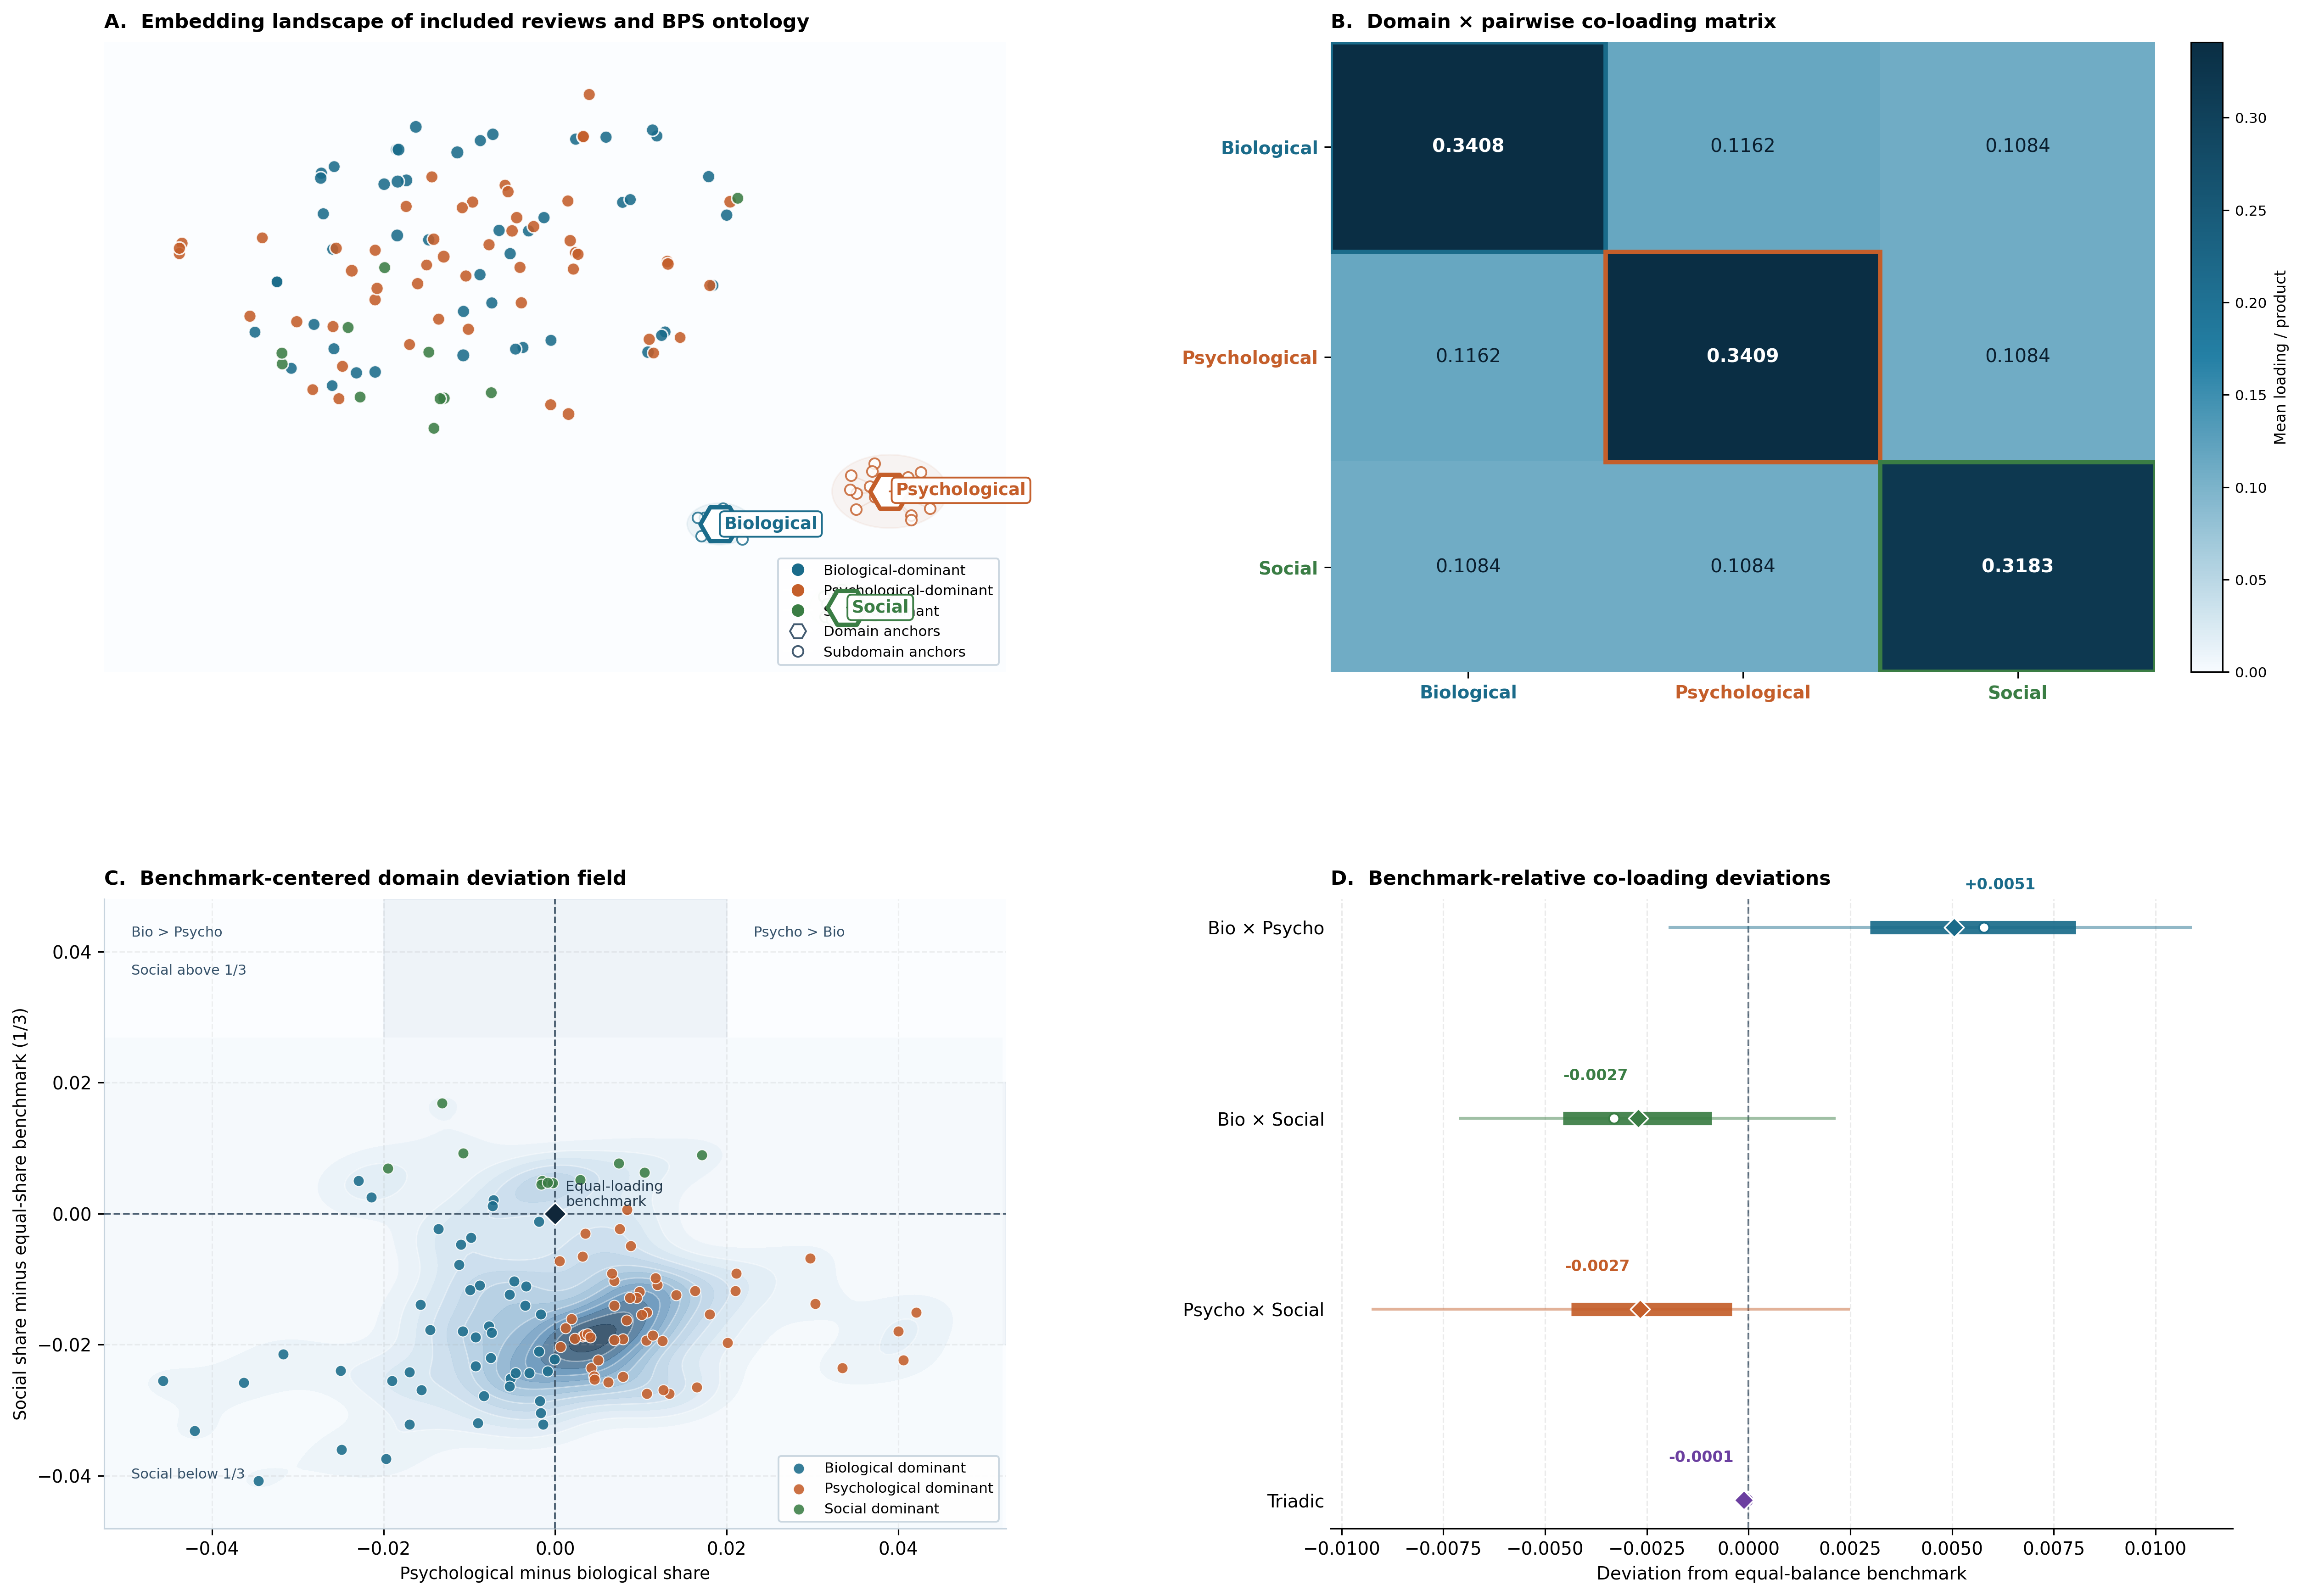
\includegraphics[width=0.99\textwidth]{../assets/figures/semantic_landscape_integrated.png}
  \caption*{\textit{Note.} Panel~A: embedding landscape of 111 included reviews (filled circles, coloured by dominant domain), domain anchors (hexagons), and 42 subdomain anchors (open circles connected to parent domains); subdomain anchors are domain-clustered for interpretability while preserving within-domain geometry after projection; background density and contour lines show the review manifold; point size scales with dominant loading strength. Projection uses PCA-preconditioned t-SNE on the joint record-plus-ontology embedding space. Panel~B: symmetric domain × pairwise co-loading intensity matrix (cell values = means). Panel~C: benchmark-centered deviation field mapping each record onto the psycho$-$bio axis (horizontal) and social benchmark deviation (vertical), with shaded near-balance bands around zero. Panel~D: benchmark-relative co-loading deviations for each pairwise and triadic term (observed minus equal-balance benchmark); bars show IQR, diamonds show means.}
\end{figure}

\subsection{Psychological Concepts and Frameworks}
\label{subsec:rq3}

Addressing \ref{rq3}, Stage~2 abstract-level extraction identified the most frequently occurring psychological construct terms. The concept profile reveals a markedly concentrated pattern: depression (27.5\%), stress (23.8\%), and anxiety (20.0\%) together account for more than 70\% of detected concept occurrences. Coping strategies (8.8\%), catastrophizing (5.0\%), and fear-avoidance (5.0\%) follow as a secondary cluster, while self-efficacy (3.8\%), resilience (2.5\%), acceptance (2.5\%), and illness perception (1.2\%) appear at lower frequencies.

This distribution supports study hypothesis H5 about conceptual clarity. The dominance of general affect labels (depression, anxiety, stress) relative to theoretically specific constructs (catastrophizing, fear-avoidance, self-efficacy) suggests that chronic pain review literature characterizes the psychological domain through symptom burden rather than through the BPS-grounded motivational, cognitive, and self-regulatory mechanisms that have the strongest theoretical support \citep{vlaeyen2000, vlaeyen2012, mccracken2014, bandura1977, sullivan1995}. Stage~3 full-text coding will map construct definitions, hierarchical relationships, and theoretical framework membership for the musculoskeletal subset.

\subsection{Conceptual Problems in BPS Usage}
\label{subsec:srq1}

\noindent\textbf{Conceptual Problems in BPS Usage.} From 111 Stage~2 records, 81/111 (73.0\%) contained at least one non-none conceptual-problem flag. At the occurrence level (multi-label flags; not mutually exclusive), 180 flags were recorded in total. The highest-frequency provisional flags were: parallel\_listing\_without\_integration (48; 26.7\%); mechanistic\_absence (46; 25.6\%); missing\_biology (33; 18.3\%); tokenistic\_bps (26; 14.4\%); vague\_definition (21; 11.7\%). The most frequent single flag was \textit{parallel\_listing\_without\_integration}. Taken together, this pattern indicates that BPS terminology is often accompanied by parallel domain listing and limited mechanistic specification, with additional signals of tokenistic framing and uneven domain coverage. These indicators are treated as hypothesis-generating and provisional until Stage~3 full-text adjudication confirms or revises them at full-text depth.


\subsection{Full-Text Retrieval Status and Stage 3 Readiness}

Of the 92 records identified as Stage~3 candidates (musculoskeletal and unspecified pain reviews), 29 (31.5\%) were retrieved as open-access full texts from PubMed Central, while 63 (68.5\%) remain in the manual retrieval queue. The 29 retrieved texts are ready for full-text deep coding once the Stage~3 codebook has been finalized through pilot testing. Completion of the manual retrieval queue is the principal dependency for full inferential closure on \ref{rq2}. To align with the OSF protocol requirement that eligibility and coding remain human-adjudicated, all candidate records are additionally listed in a manual relevance audit sheet with reviewer and adjudication fields.

% ============================================================
\section{Discussion}
\label{sec:discussion}

\subsection{The BPS Model as Label versus Framework}

The central finding is an asymmetry between the frequency of BPS language use and the depth of its operationalization. Across 111 included reviews, provisional typological coding classified 65.8\% as pseudo-BPS or partial-signal and 15.3\% as rhetorical label signal, while only 9.0\% reached a potential integrative signal and 9.9\% a multifactorial signal. The resulting picture indicates that explicit triadic integration signals are comparatively uncommon at abstract level.

The concern is not strategic dishonesty. BPS language is semantically broad enough to invoke without specifying what integration entails: which pathways connect the domains, in which directions, at which time scales. The provisional typology developed here gives this critique empirical grip. A record is coded as potential integrative signal only if it (a) covers all three domains and (b) declares an explanatory framework or organizing principle function---the minimum abstract-level signal of intended integration. That roughly four in five records fail this criterion is a precise, auditable claim, not a subjective impression \citep{borrell2004, wade2017}. This finding provides confirmatory evidence for study hypothesis H1.

\subsection{The Social Domain Deficit}

Perhaps the most striking finding is the systematic underrepresentation of social factors across both structured abstract-level coding and semantic loading. In the substantive coding layer, social factors were present in 56.0\% of musculoskeletal records and 48.6\% of the full corpus, yet semantic loading ranked social as dominant in only 9.9\% of records (versus 46.8\% psychological, 43.2\% biological). The mean social loading (0.318) was lower than both biological (0.341) and psychological (0.341). The pattern holds across methods.

This social loading deficit is interpretable as a systematic pattern in which the ``S'' of BPS is lexically present but conceptually thin---named without the mechanistic or operational specification that biological factors receive through neuroimaging, pharmacology, or genetics, and psychological factors through standardized measurement instruments and theoretical models \citep{dorner2011, harkness2005, edwards2016}. Social determinants (socioeconomic status, occupational context, medicolegal systems, cultural factors) appear in review discourse as labels rather than as substantively operationalized constructs with defined pathways. This confirms study hypothesis H3. Stage~3 integration coding will allow this to be tested against full-text evidence, but the convergence between two independent measurement strategies is a robust preliminary signal.

\subsection{Psychological Construct Concentration and the Affect Paradox}

The psychological concept distribution---dominated by depression, anxiety, and stress, with limited representation of specific cognitive and self-regulatory constructs---reveals a tension in the pain psychology literature. The theoretical foundations of BPS-aligned pain psychology emphasize specific mechanisms: catastrophizing as a cognitive amplifier of pain \citep{sullivan1995}; fear-avoidance as an operant-conditioning pathway from acute to chronic pain \citep{vlaeyen2000, vlaeyen2012}; illness beliefs as interpretive frames that shape help-seeking and treatment adherence; and self-efficacy as a cross-cutting mediator of functional outcomes \citep{bandura1977}. Yet the abstract-level concept profile suggests that emotionally oriented general labels dominate how psychological factors are represented in review summaries.

Two interpretations are possible. First, this may be a reporting artefact: abstracts may prioritize outcome-relevant affect labels (depression, anxiety) that are measured by standard instruments, while theory-specific constructs are detailed in the full text. Second, the pattern may reflect a genuine preponderance of affect-focused framing in BPS pain reviews, consistent with meta-analytic findings showing that CBT and interdisciplinary interventions primarily target depressive and anxiety symptoms \citep{morley1999, williams2020}. Distinguishing these explanations---artefact or signal---is a primary motivation for Stage~3 deep coding.

\subsection{Semantic Loading as a Methodological Contribution}

The ontology-aligned semantic loading procedure developed here extends structured abstract-level content coding in three ways. First, it is continuous and multi-dimensional: each record receives a domain loading profile rather than a binary domain-mention indicator, capturing graded orientation rather than presence/absence. Second, the subdomain resolution (42 categories) maps specific research constructs within each domain, allowing detection of which biological subdomains (e.g., pharmacological treatment vs.\ central sensitization) or psychological subdomains (e.g., CBT approaches vs.\ fear-avoidance) dominate a record's semantic space. Third, the pairwise product terms measure co-loading intensity as an approximation of conceptual overlap between domains, providing a text-derived integration signal that complements the binary triadic co-mention indicator.

The social deficit finding illustrates the procedure's sensitivity: while structured abstract-level coding still shows near-universal social mention, semantic loading shows social dominant in only 9.9\% of records, exposing the gap between mentioning and substantively organizing a review around social factors. This methodological contribution---surfacing the qualitative-quantitative divergence between surface-level mention and semantic orientation---is generalizable to other conceptual systematic reviews in pain science and beyond.

\subsection{Methodological Limitations}

The principal limitation is the interim status of the synthesis. Stage~3 full-text coding remains incomplete, constraining inferential closure on integration quality, construct-level mapping, and balance assessment. The absence of completed manual retrieval for 57 records limits Stage~3 candidate coverage. PsycINFO was not available for this run, which may underrepresent reviews indexed primarily in psychology databases. The provisional typological scheme relies on abstract-level signals and may misclassify records whose integration quality is only apparent in the full text. Finally, the semantic loading procedure is sensitive to ontology term selection; the current 42-subdomain scheme reflects one operationalization among possible alternatives, and results should be interpreted relative to this specific ontological framing.

This synthesis represents a high-fidelity interim analysis pending Stage~3 full-text coding and dual-coder adjudication. The search covered MEDLINE and Web of Science; PsycINFO records were not available for this run due to credential constraints, which may underrepresent reviews indexed primarily in psychology databases. Stage~3 full-text retrieval is incomplete (53/87 in manual queue), constraining inferential closure on domain integration quality. The provisional typology relies on abstract-level signals and may misclassify records whose integration quality is apparent only in full text. Semantic loading is sensitive to ontology term selection; the 42-subdomain scheme reflects one operationalization among possible alternatives.


\subsection{Implications for Research Practice and Reporting Standards}

The findings have actionable implications. Future chronic pain reviews that invoke the BPS model should provide explicit reporting of: which domains are covered; how domain interactions are conceptualized; what mechanistic pathways are proposed; and whether theoretical framework claims are supported by the review's empirical content. A practical proposal is that journals adopt mandatory reporting prompts distinguishing rhetorical from substantive BPS integration, modelled on existing PRISMA extensions \citep{page2021}. Editorial and peer-review practices that currently accept BPS invocation as self-evidently legitimate would benefit from standardized criteria distinguishing descriptive domain listing from mechanistic triadic integration.

% ============================================================
\section{Conclusion}
\label{sec:conclusion}

This systematic review provides the first comprehensive empirical map of how the biopsychosocial model is operationalized across 111 eligible chronic pain review articles spanning 1990 to 2026. The evidence indicates that BPS language is ubiquitous but operationally uneven: many reviews still demonstrate domain listing or partial coverage rather than mechanistic triadic integration; social factors are consistently underspecified relative to psychological and biological ones in the semantic-loading layer; and the psychological construct profile is dominated by general affect labels rather than the specific cognitive and self-regulatory mechanisms that BPS-aligned theories emphasize. Convergent evidence from two independent methods---structured Stage~2 coding and ontology-aligned semantic loading---strengthens confidence in the social deficit and psychological concentration findings. These results are currently provisional, pending Stage~3 full-text coding of the musculoskeletal subset and dual-coder adjudication. Final inferential claims about integration quality and construct-level framework architecture await completion of manual retrieval and the PsycINFO search. The staged, auditable pipeline and reproducible ontology-based semantic analysis developed here provide the infrastructure for that completion and a template for future conceptual systematic reviews in pain science.

% ============================================================
\section*{Data and Code Availability}
\label{sec:datacode}

\begin{sloppypar}
Analysis code, pre-registration materials, and supplementary data are openly available.\\
\textit{Pre-registration} (protocol, search strings, codebooks, and audit trail):
\url{https://osf.io/t4fam/overview} (DOI:~10.17605/OSF.IO/T4FAM; \citealt{osfprotocol2026}).\\
\textit{Code repository} (full pipeline, embedding analysis, and figure generation):
\url{https://github.com/stvsever/SystematicReview_on_BioPsychoSocialModel_in_ChronicPainReseach}.
\end{sloppypar}

% ============================================================
\bibliographystyle{plainnat}
\bibliography{references}

\clearpage
\appendix
\section{Supplementary Methods}
\label{app:methods}
Supplementary Methods Note. Protocol alignment and reliability.

Operational pipeline stages preserve the pre-registered sequencing while logging deviations explicitly. Stage~2 uses structured LLM-based abstract coding with deterministic metadata fields and archived batch outputs; this augments rather than replaces final adjudication. Dual-coder templates are generated for Stage 1, Stage 2, and Stage 3 reliability checks, consistent with the registered subset reliability design. Current reliability file status.
stage1. status=not\_ready, n=0, percent\_agreement=, kappa=
stage2. status=not\_ready, n=0, percent\_agreement=, kappa=
stage3. status=not\_ready, n=0, percent\_agreement=, kappa=

Semantic loading note. Ontology-aligned embeddings generated through OpenRouter.


\section{Supplementary Semantic Tables}
\label{app:semantic}
\begin{table}[htbp]
\raggedright
\caption{Ontology-based semantic loading summary across BPS domains.}
\label{tab.semantic.summary}
\begin{tabular}{lllr}
\toprule
domain & mean\_cosine & mean\_loading & dominance\_n \\
\midrule
biological & 0.5221 & 0.3408 & 48 \\
psychological & 0.5224 & 0.3409 & 52 \\
social & 0.4534 & 0.3183 & 11 \\
\bottomrule
\end{tabular}

\caption*{Note. Method=openrouter\_embedding; model=openai/text-embedding-3-small. Mean loading uses softmax-normalized cosine similarity.}
\end{table}

\begin{table}[htbp]
\raggedright
\caption{Pairwise and triadic semantic integration summary.}
\label{tab.semantic.pairwise.summary}
\begin{tabular}{rrrr}
\toprule
bio\_psych\_mean & bio\_social\_mean & psych\_social\_mean & triadic\_product\_mean \\
\midrule
0.116200 & 0.108400 & 0.108400 & 0.036900 \\
\bottomrule
\end{tabular}

\caption*{Note. Pairwise scores are products of normalized domain loadings per record.}
\end{table}


\noindent The full subdomain loading summary (42 subdomains) is archived at:\\
\texttt{paper/assets/tables/semantic\_subdomain\_summary.csv}.

\section{Supplementary Catalog of Included Reviews}
\label{app:catalog}
The complete Stage~2 included review catalog is provided as a machine-readable supplementary file:
\texttt{paper/assets/tables/included\_review\_catalog.csv}. Key fields are described in the registered codebook available at the repository listed in the Data and Code Availability section.

\end{document}
